%%%--- Template for master thesis at SfS
%%%--- Modified template with more comments and examples -- SG, 11/06/09
%%%------
\documentclass[11pt,a4paper,twoside,openright]{report}
%%not needed \usepackage{E}
\usepackage[english]{ETHDAsfs}%--> ETHDASA + fancyheadings + ... "umlaute"
%  + sfs-hyper -> hyperref

\usepackage{tikz}
\usepackage{pdflscape}
\usepackage{pdfpages}
\usepackage{graphicx}

\usepackage{hyperref}
\usepackage{pdfpages}%%to include the confirmation of originality (plagiarism
\usepackage{amsbsy}%% for \boldsymbol and \pmb{.}
\usepackage{amssymb}%% calls  amsfonts...
%or \usepackage{german8}%-- =  german  +  isolatin1
\usepackage{graphicx}%-- f�r PostScript-Grafiken (besser als  psfig!)
%\usepackage[draft]{graphicx} % grafics shown as boxes --> faster compilation
% \addbibresource{biblio.bib}

\usepackage[longnamesfirst]{natbib}%was {sfsbib}%- F�r  Literatur-Referenzen
%           ^^^^^^^^^^^^^^ 1) "Hampel, Ronchetti, ..,"  2) "Hampel et al"
% Engineers (and other funny people) want to see [1], [2]
% ---> use 'numbers' : \usepackage[longnamesfirst,number]{natbib}
%
%
\usepackage{texab}%- 'tex Abk�rzungen' /u/sfs/tex/tex/latex/texab.sty
        %%- z.B.  \R, \Z, \Q, \Nat f�r reelle, ganze, rationale, nat�rl. Zahlen;
        %%-       \N   (Normalvert.)  \W == Wahrscheinlichkeit .....
        %%-  \med, \var, \Cov, \....
        %%-  \abs{x} == |x|   und   \norm{y} ==  || y ||   (aber anst�ndig)
%% NOTE: texab contains many useful definitions and "shortcuts". It is
%% worth to open the file and have a look at them. HOWEVER, some
%% definitions are a bit can lead to conflicts with other packages. You
%% might for example want to comment out the line defininf \IF as an
%% operator when working with the algorithmic package, or to comment out
%% the line defining a command \Cite with working with the Biblatex package
\usepackage{amsmath}
%\usepackage{mathrsfs}% Raph Smith's Formal Script font --> provides \mathscr
\usepackage{enumerate}% Fuer selbstdefinierte Nummerierungen
%--------
\usepackage{relsize}%-> \smaller (etc) used here
\usepackage{color} %% to allow cloring in code listings
\usepackage{fancyvrb}% Fuer R-code, C-code, ....  and settings for these:
\usepackage{listings}% Fuer R-code, C-code, ....  and settings for these:
\definecolor{Mygrey}{gray}{0.75}% for linenumbers only!
\definecolor{Cgrey}{gray}{0.4}% for comments
\lstloadlanguages{R}
\lstset{ %% Hilfe unter z.B. http://en.wikibooks.org/wiki/LaTeX/Packages/Listings
language=R,
basicstyle=\ttfamily\scriptsize,%%- \small > \footnotesize > \scriptsize > \tiny
%commentstyle=\ttfamily\color{Cgrey},
commentstyle=\itshape\color{Cgrey},
numbers=left,
numberstyle=\ttfamily\color{Mygrey}\tiny,
stepnumber=1,
numbersep=5pt,
backgroundcolor=\color{white},
showspaces=false,
showstringspaces=false,
showtabs=false,
frame=single,
tabsize=2,
captionpos=b,
breaklines=true,
%breakatwhitespace=false,
keywordstyle={},
morekeywords={},
xleftmargin=4ex,
literate={<-}{{$\leftarrow$}}1 {~}{{$\sim$}}1}
\lstset{escapeinside={(*}{*)}} % for (*\ref{ }*) inside lstlistings (Scode)
%%----------------------------------------------------------------------------

%%------- Theoreme ---
\newtheorem{definition}{Definition}[subsection]
\newtheorem{lemma}[definition]{Lemma}
\newtheorem{theorem}[definition]{Theorem}
\newtheorem{Coro}[definition]{Corollary}
\theoremstyle{definition}
\newtheorem{example}[definition]{Example}
\newtheorem*{note}{Note}
\newtheorem*{remark}{Remark}

\DeclareMathOperator*{\plim}{plim}
% \def\MR#1{\href{http://www.ams.org/mathscinet-getitem?mr=#1}{MR#1}}

% \newcommand{\Lecture}[3]{\marginpar{#3.#2.#1}}
% \newcommand{\Fu}{\mathcal{F}}
\newcommand{\aatop}[2]{\genfrac{}{}{0pt}{}{#1}{#2}}

%\renewcommand{\theequation}{\arabic{equation}}
\numberwithin{equation}{chapter}

%%%%%%%%%%%%%%%%%%%%%%%%%%%%%%%%%%%%%%%%%%%%%%%%%
%%% Path for your figures                      %%%
%%%%%%%%%%%%%%%%%%%%%%%%%%%%%%%%%%%%%%%%%%%%%%%%%
% Set the paths where all figures are taken from:
% \graphicspath{{Pictures/}}
\graphicspath{{../../plot/}}

%%%%%%%%%%%%%%%%%%%%%%%%%%%%%%%%%%%%%%%%%%%%%%%%%
%%% Define your own commands here             %%%
%%%%%%%%%%%%%%%%%%%%%%%%%%%%%%%%%%%%%%%%%%%%%%%%%
\newcommand{\Bruch}[2]{{}^{#1}\!\!/\!_{#2}}
\renewcommand{\labelenumi}{\roman{enumi}.)}

%%%%%%%%%%%%%%%%%%%%%%%%%%%%%%%%%%%%%%%%%%%%%%%%%
%%% Listings parameters
%%%%%%%%%%%%%%%%%%%%%%%%%%%%%%%%%%%%%%%%%%%%%%%%%
\usepackage[dvipsnames]{xcolor}
\xdefinecolor{lightgray}{RGB}{247, 247, 247}% R's col2rgb("gray97"); #F7F7F7
\xdefinecolor{semilightgray}{RGB}{240, 240, 240}% R's col2rgb("gray94"); #F0F0F0
\xdefinecolor{middlegray}{RGB}{127, 127, 127}% R's col2rgb("gray50"); #7F7F7F
\xdefinecolor{seashell}{RGB}{255, 245, 238}% R's col2rgb("seashell"); "#FFF5EE"
\xdefinecolor{yellow}{RGB}{255, 255, 128}% R's self-defined (weakened yellow); #FFFF80
\xdefinecolor{orange}{RGB}{238, 118, 0}% R's col2rgb("darkorange2"); #EE7600
\xdefinecolor{red}{RGB}{178, 34, 34}% R's col2rgb("firebrick"); #B22222
\xdefinecolor{blue}{RGB}{58, 95, 205}% R's col2rgb("royalblue3"); #3A5FCD
\xdefinecolor{deepskyblue}{RGB}{0, 154, 205}% R's col2rgb("deepskyblue3"); #009ACD
\xdefinecolor{chocolate}{RGB}{205, 102, 29}% R's col2rgb("chocolate3"); #CD661D
\newcommand*{\gray}[1]{\textcolor{gray}{#1}}
\newcommand*{\seashell}[1]{\textcolor{seashell}{#1}}
\newcommand*{\yellow}[1]{\colorbox{yellow}{#1}}
\newcommand*{\orange}[1]{\textcolor{orange}{#1}}
\newcommand*{\red}[1]{\textcolor{red}{#1}}
\newcommand*{\blue}[1]{\textcolor{blue}{#1}}

% general listings settings
% see http://tex.stackexchange.com/questions/94238/listings-general-settings-for-a-language-seem-to-be-overwritten-not-respected/94242#comment201538_94242
\lstset{% these settings are used for *all* listings
  basicstyle=\ttfamily\small,% basic font style
  frame=lrtb, framerule=0pt, framexleftmargin=1pt,% put some space around the shade
  basewidth=0.5em,% smaller base width of a character
  tabsize=8,% sizes of tabs
  showstringspaces=false,% do not replace spaces in strings by a certain character
  captionpos=b,% positioning of the caption below
  breaklines=true,% automatic line breaking
  % escapeinside={(*}{*)},% escaping to LaTeX => EVIL since str() may produce
  % "(*" which is then escaped... )
  fancyvrb=true,% verbatim code is typeset by listings
  extendedchars=false,% prohibit extended chars (chars of codes 128--255)
  rangeprefix=\#\#'\ \{\ ,% marker opening symbol
  rangesuffix=\ \},% marker closing symbol
  includerangemarker=false,% hide markers
  backgroundcolor=\color{semilightgray},% background color
  commentstyle=\itshape\color{chocolate},% comment style
  keywordstyle=\color{blue},% keyword style
  stringstyle=\color{deepskyblue},% string style
  numbers=left,% display line numbers on the left side
  numberstyle=\color{middlegray}\tiny% use small line numbers
}

% lower priority settings (should be used first in lstlisting environments; will
% be overwritten by the language specific settings if both are given)
\lstdefinestyle{input}{
  backgroundcolor=\color{semilightgray},% background color
  commentstyle=\itshape\color{chocolate},% comment style
  keywordstyle=\color{blue},% keyword style
  stringstyle=\color{deepskyblue},% string style
  numbers=left,% display line numbers on the left side
  numberstyle=\color{middlegray}\tiny% use small line numbers
}
\lstdefinestyle{output}{
  backgroundcolor=\color{lightgray}% background color
}

% listings settings for LaTeX (note: TeX dialects don't have keywords but texcs's)
\lstdefinestyle{Lstyle}{
  language=[LaTeX]TeX,% set programming language
  texcs={},% texcs
  otherkeywords={}% undefine otherkeywords
}

% LaTeX input with listings
\lstnewenvironment{Linput}[1][]{%
  \lstset{style=input, style=Lstyle}
  #1% content
}{\vspace{-0.25\baselineskip}}% note: -\baselineskip leads to no space

% LaTeX output with listings
\lstnewenvironment{Loutput}[1][]{%
  \lstset{style=output, style=Lstyle}
  #1% content
}{\vspace{-0.25\baselineskip}}% note: -\baselineskip leads to no space

% listings settings for R
\lstdefinestyle{Rstyle}{
  language=R,% set programming language
  literate={<-}{{$\bm\leftarrow$}}2{<<-}{{$\bm{\mathrel{\bm\leftarrow\mkern-14mu\leftarrow}$}}}2{<=}{{\raisebox{0.6pt}{\scalebox{0.8}{$\bm\le$}}}}2{>=}{{\raisebox{0.6pt}{\scalebox{0.8}{$\bm\ge$}}}}2{!=}{{$\bm\neq$}}2,% item to replace, text, length of chars
  keywords={if, else, repeat, while, function, for, in, next, break},% keywords; see R language manual, /usr/local/texlive/2012/texmf-dist/tex/latex/listings/lstlang3.sty
  otherkeywords={}% undefine otherkeywords to remove !,!=,~,$,*,\&,\%/\%,\%*\%,\%\%,<-,<<-,_,/
}


\newcommand{\insertplot}[2]{
  \begin{figure}[!ht]
    \centering
    \input{tex_output/#1}
    \caption{#2}
  \end{figure}
}

\newcommand{\insertmodel}[2]{
  \input{tex_output\#1}
}


%%%%%%%%%%%%%%%%%%%%%%%%%%%%%%%%%%%%%%%%%%%%%%%%%
%%% End of listing parameters
%%%%%%%%%%%%%%%%%%%%%%%%%%%%%%%%%%%%%%%%%%%%%%%%%
\begin{document}
\bibliographystyle{chicago}% ---> Hampel,F., E.Ronchetti,... W.Stahel(1986) ...
 %was \bibliographystyle{sfsbib}\citationstyle{dcu} %OR DEFAULT : \citationstyle{agsm}

\pagenumbering{roman}%- roman numbering for first few pages

%%%%%%%%%%%%%%%%%%%%%%%%%%%%%%%%%%%%%%%%%%%%%%%%%
%%% Title page                                %%%
%%%%%%%%%%%%%%%%%%%%%%%%%%%%%%%%%%%%%%%%%%%%%%%%%
\period{Fall 2015}
\dasatype{Semester Paper}
\students{David Pham}
\mainreaderprefix{Adviser:}
\mainreader{Prof.\ Jan-Egbert Sturm}
\alternatereaderprefix{Co-Adviser:}
\alternatereader{Prof.\ Norbert Hungerb�hler}
\submissiondate{March 15th 2016}
\title{Public Employment: \\
  Data Analysis with OECD Economic Outlook Quarterly Data}

\maketitle%- Titelseite wird abgeschlossen
\cleardoublepage
 %%~~~~~~~~~~~~~~~~~~~~~~~~~~~~~~~~~~~~~~~~

\linespread{1.5}\selectfont

%%%%%%%%%%%%%%%%%%%%%%%%%%%%%%%%%%%%%%%%%%%%%%%%%
%%% Insert here acknowledgements and abstract %%%
%%%%%%%%%%%%%%%%%%%%%%%%%%%%%%%%%%%%%%%%%%%%%%%%%
%% Dedication (optional)
\markright{}
\vspace*{\stretch{1}}
\begin{center}
  To Myriam for her support during the long nights of work and to our future
  children.
\end{center}
\vspace*{\stretch{2}}

% % Preface (optional)
% \newpage
% \markboth{Preface}{Preface}
% \chapter*{Preface}

First words and acknowledgements.

%%% Local Variables: 
%%% mode: latex
%%% TeX-master: "MasterThesisSfS"
%%% End: 


% Abstract should not be longer than one page.
\newpage
\markboth{Abstract}{Abstract}
\include{abstract}

%%%%%%%%%%%%%%%%%%%%%%%%%%%%%%%%%%%%%%%%%%%%%%%%%
%%% Table of contents and list of figures and %%%
%%% tables (no need to change this usually)   %%%
%%%%%%%%%%%%%%%%%%%%%%%%%%%%%%%%%%%%%%%%%%%%%%%%%
\newpage
\tableofcontents
\newpage
\listoffigures
\newpage
\listoftables

%% Notations and glossary (optional)
% \cleardoublepage
% \phantomsection
% \addcontentsline{toc}{chapter}{\protect\numberline{}{Notation}}
% \markboth{Notation}{Notation}
% % \chapter*{Notation}
% \label{c:Notation}

% Explain your symbols and abbreviations.

%%% Local Variables:
%%% mode: latex
%%% TeX-master: "MasterThesisSfS"
%%% End:


\cleardoublepage
\pagenumbering{arabic}%--- switch back to standard numbering


%%%%%%%%%%%%%%%%%%%%%%%%%%%%%%%%%%%%%%%%%%%%%%%%%
%%% Your text... Either write here directly,  %%%
%%% or even better: write in separate files   %%%
%%% that you just have to include here.       %%%
%%%%%%%%%%%%%%%%%%%%%%%%%%%%%%%%%%%%%%%%%%%%%%%%%
\chapter{Introduction}

Since the start of the 2008 financial crisis, countries and governments heavily
have relied on their respective central banks to boost their economies and
support growth. Thanks to low interest rates, governments and their leaders
could probably invest in the economy and provide employment to the
population. They can provide it by several means: keeping a low corruption,
creating an employment friendly environment and naturally employ professionals
directly, the so-called public servants.

The share of civil servants with respect to total labor force varies over time,
and several hypothesis exist to explain why. One of the recurring idea is that
incumbent governments have incentives to increase the number of civil servants
before elections to raise their chances of reelection and this would be easier
in environment where fiscal transparency is low.

The purpose of this semester paper is to synthesize the current literature of
the subject, and most importantly to gather and to prepare data for a
replication of the results of the literature by using quarterly data
from the OECD Economic Outlook.

The added value of this work is that a quarterly data set is used as input to
study the problem. This would be for the first time, to the best of our
knowledge. The main challenge to complete the work has been to gather the data,
to tidy them and to merge them. Moreover, as the data set contains hundreds of
observational variables, statistical analysis should be executed cautiously.

With modern technology, studies should be as transparent and reproducible as
possible. Hopefully, the Github
repository\footnote{\url{https://github.com/davidpham87/public_employment_analysis}}
of the project offers full transparency over the data and the code used to
handle them. The analysis is performed with the statistical environment
\textsf{R} (\cite{R2015}) and the main scripts to perform the analysis is supplemented in the
appendix.

The structure of the semester paper is following: a first part is devoted to
summarize the research of recent papers, then it focuses on the statistical
analysis of the data, before concluding.

%%% Local Variables:
%%% mode: latex
%%% TeX-master: "semester_paper_sfs"
%%% End:

\section{Theory}\label{Theory}

This section synthesizes three papers used as theoretical background to run our
analysis. These are:

\begin{enumerate}
\item \cite{alesina2000redistributive}, which studies American states about
  their election and in order to find if any inequality measures could predict
  the share of public servants.
\item \cite{alt2014isn}, that describes the effect of accounting practices of
  EU countries over public employment.
\item \cite{aaskoven2015fiscal}, which analyzes the effect fiscal transparency
  on civil servants.
% \item \cite{schuster2013retreat} studies the retreat of OECD countries from the
%   sectors. The most notable quality of this paper is the data set they
%   collected across the countries and the years.
\end{enumerate}

\section{Theoretical models}

\cite{alesina2000redistributive} supposes that American cities use public
employment as a discreet mean for wealth redistributing: It channels resources
from middle class voters to disadvantaged citizens when an explicit
tax-transfer scheme would not find political support. In order to justify their
idea, they set the following theoretical framework: define a two periods
time-frame, with an election after the first period. There are two classes of
voters (\emph{middle} class and the \emph{poor}) and two contestants for the
government. Each candidate need the support of the middle class in order to win
the election. The challenge of the incumbent government is to know whether it
should start a public project to employ people from the poor class, at the risk
of losing political support from the middle class.

Define \(B\) as the benefit of a public project. This benefit can be thought of
the employment of the \emph{poor} to complete the project. Then restrict $B$ to
a discrete random variable with
\begin{align*}
  B =
  \left\{
    \begin{array}{ll}
    B_L & \mbox{with probability } 1-\theta \\
    B_H & \mbox{with probability } \theta
    \end{array}
  \right.
\end{align*}

where $0 < B_L < B_H$ and \(\theta\) is random variable taking either
\(\theta_L\) or \(\theta_H\) with \(0 < \theta_L < \theta_H < 1\). When
\(\theta=\theta_L\), it is more efficient to make a cash transfer than
implementing the project. Intuitively, $\theta$ is the risk of the
project. Moreover, the incumbent government observes the realisation of
\(\theta\) before deciding to implement a public project or not.

As there are two contestants for the government they also possess different
preferences: one supports the middle class and conduct the public project only
if \(\theta = \theta_H\), whereas the other favors the poor, leading the public
project for any value of \(\theta\) as long as the latter action does not
prevent the candidate from winning the next election.  Voters do not know which
type are the politicians, but they have prior believes: they are not completely
certain whom the candidates support. Moreover, being reelected is always
favored by the incumbent candidate as it maximizes her utility.

Under these conditions, \cite{alesina2000redistributive} shows there exists an
optimal decision for the incumbent government given $\theta$ and its
preferences. With the appropriate data, the paper observes that several
inequality measures are correlated with public employment shares, hence
supporting their view.

\cite{alt2014isn} and \cite{aaskoven2015fiscal} have a similar hypothesis: the
incumbent government will boost the share of public employment as election
dates are nearing in order to stay elected. They assert that the magnitude of
these changes can be explained by the degree of fiscal transparency of the
governments. Fiscal transparency is often measured measured by evaluating the
quality and frequency of financial reports from a country. They assume that
fiscal opacity allows governments to use unorthodox accounting methodology to
please political partners, financial markets and voters. It also allows them to
use use windfall revenues to employ more civil servants without voters
noticing, even though if these would prefer to have a tax cut or a cash
transfer. Furthermore, increasing the number public employees is a fast and
easy process for the incumbent government, because it usually does not require
a modification in the laws or the approval of the parliament.


\section{Statistical Analysis}

In practice, two challenges were encountered during the analysis: data
interpolation and statistical analysis.

\paragraph{Data interpolation}

The Economic Outlook dataset from the OECD exists in annual and quarterly
frequencies. Nevertheless, numerous variables are not measured quarterly and
quarterly interpolation of annual data is a reasonable choice in order to
retain information. However, economists often require for level variables
(i.e. measure with units) that the sum of quarterly data to be equal to the
annual value.  \cite{sax2014tempdisagg} proposes the Denton(-Chollette) method
as a decent choice for performing such a task. Heuristically, this method
(so-called temporal distribution or \emph{disaggregation}) solves the problem
by dividing and spreading the annual value into quarterly values, such that the
interpolation looks smooth in the end. This process can be thought as a smart
spline interpolation adjusted by a scaling factor. More sophisticated
methodology might use correlated quarterly variables in order to adjust the
annual ones, but this usually leads to over-fitting.

\paragraph{Data analysis}

The standard statistical methods in the literature are the regular multiple
linear regression. The cited references use the a common model. Assume that
$Y_{it}$ denotes the public employment rate (number of civil servants over
total labor force) for the $i$-th country and time $t$. Then $Y_{it}$ is fitted
as
\begin{align} \label{eq:reg}
  Y_{it} = X_{it}\beta + \eta_i + \tau_t + \varepsilon_{it}, \quad i \in \{1, \dots, n\},\ t \in \{1, \dots, T\},
\end{align}
where $X_{it} \in \mathbb{R}^{n \times p}$ is a matrix of explanatory and
control variables, $\beta \in \mathbb{R}^{p}$ is the regression coefficient,
$\eta_i$ is a country fixed-effect and $\tau_t$ is a time-fixed effect,
$\varepsilon_{it}$ are non-correlated centered gaussian random variables, $n$,
respectively $T$, is the number of countries, respectively, period of
observations. One weakness in the analysis of the literature is that
assumptions of the multiple regression are seldom checked. This is problematic
as for our data set the fitted values of $\varepsilon_{it}$ and
$\varepsilon_{i(t+1)}$ are highly correlated, contradicting the
assumption. Additionally, statistical significance is often reported with raw
$p$-values. Nonetheless, using these unprocessed $p$-values leads to a higher
rate of false positive. Best practice recommend to adjust these by controlling
the false discovery rate (see \cite{benjamini1995controlling}).

%%% Local Variables: ***
%%% mode:latex ***
%%% TeX-master: "semester_paper_sfs.tex"  ***
%%% End: ***
%%% reftex-default-bibliography: ("biblio.bib")
 % theoretical background
\chapter{Empirical Analysis}

This chapter is structured as such: a first section describes the data and its
variables, their source and a reason to incorporate them in the analysis. This
is followed by a presentation of the results and their analysis.

\section{Data}

The main data comes from the OECD Economic Outlook ($98^{th}$ edition)
(cf. \cite{oecd2015eo}) with annual and quarterly frequency. We only use a
subset of the data set with the following variables.
\begin{itemize}
\item Public employment rate of OECD countries between 1990 to 2012. Public
  employment rate is defined as the number of civil servant divided by the
  total labor force. Figure \ref{fig:egr} shows the public employment rate used
  for the data analysis.
\item Unemployment rate in percent. Everything else being equal, the
  correlation with public employment rate should be negative: the total labor
  force is composed of employed plus unemployed people, hence if the number of
  workers in the private industry remain stable, a diminishing unemployment
  rate should increase the public employment rate.
\item Government revenues in percent of GDP: the share of GDP that the
  government receive from taxes and others sources of income. This variable
  captures the size of the government.
\item Net lending in percent of GDP: the difference between revenues and
  expenditures scaled by GDP. The net lending captures how well the incumbent
  government manages its budget.
\item GDP Growth in percent. It is believed that this variable represent the
  effect economic cycle and momentum in an economy.
\item GDP per capita in 2010 USD Purchasing power parity, in order to control
  for the Wagner's Law, stating that richer populations care more about common
  goods (often provided by government). The effect of wealth over the public
  employment share should be non-linear, reason for which its $\log$ is used in
  the models.
\end{itemize}

Moreover, the following time series have been collected to test the assertion
of the literature.
\begin{itemize}
\item The 105 election quarters for the relevant OECD countries were recorded
  from Wikipedia (\cite{wiki2015election}); From the election dates, one can
  deduce the number of years until the normal end of the term.
\item Fiscal transparency score, \cite{wang2015trends} from the IMF. A low
  fiscal transparency allows governments to use windfall revenues to boost the
  number of public employees or to adjust their national accounts.
\item Political direction of the executive government (left or right) from the
  World Bank (\cite{beck2001new}). One desires to capture the effect or
  correlation of the political partisanship over public employment rate. It
  should be increased when a left-wing governments is elected.
\item Gini coefficient, before and after tax from the Standardizing the world
  income inequality database (\cite{solt2009standardizing}). The Gini
  coefficient is a standard measure to assess the income inequality within a
  country. A high level of inequality should lead to a bigger rate of public
  employees, as a mean for the government to redistribute wealth.
\end{itemize}

Plots of these variable are showed in Appendix \ref{ch:data-viz}. We also
assumed that structural breaks could have affected the public employment rate
in the data set. \cite{james2014ecp} provides a non-parametric algorithm to
detect such point. As Figure \ref{fig:strct:breaks} depicts, although there are
some individual changes, there are no overall break at given time point. Hence
the idea has been abandoned.

\section{Analysis}

\subsection{Results}

For our analysis, we extend the model from Equation \eqref{eq:reg} with the
following equation:
\begin{align*}
  Y_{it} = \alpha Y_{i{t-1}} + X_{it}\beta + \eta_i + \tau_t +
  \varepsilon_{it} \quad i \in \{1, \dots, n\},\ t \in \{1, \dots, T\},
\end{align*}
where $X_{it}$ is the independent variable and contains the unemployment rate,
government revenues and net lending for $i$-th country at time $t$. The other
variables are similar to Equation \eqref{eq:reg}. This model, albeit
counter-intuitive, is stable and robust. Additionally, the auto-regressive
aspect reduces the correlation of the error terms $\varepsilon_{it}$.  Table
\ref{tbl:main-coeff} shows the coefficient of the regression\footnote{The
  output of linear models has produced with the Stargazer package
  (\cite{hlavac2015stargazer}) used with the statistical programming language
  \textsf{R}.}. Moreover, Figure \ref{fig:diag:lm} provides some support about
the soundness of our statistical model: the residuals of the regression seem to
be uncorrelated, although there is evidence they do not follow a Gaussian
distribution. The regression tables for the additional variables are in the
Appendix \ref{ch:reg-tbls}.  Note the following supplementary observations.


\begin{enumerate}
\item The number of fitted parameter is much bigger than what is displayed in
  the tables: one degree of freedom is allocated for each quarter to fit $\tau_t$
  (88 for the 22 years of observations) and for the country parameter $\eta_i$
  (17 parameters).
\item The main variables (unemployment rate, government revenue and net
  lending) keep the same regression coefficient and their statistical
  significance.
\item The absolute size of these coefficients are quite small.
\item GDP growth and the Gini coefficient after taxes have significant
  regression coefficient before adjustment of the $p$-values, but become
  insignificant afterwards.
\item The effect of the wealth of a nation, measured by the GDP per capita, is
  unexpectedly not correlated. This observation does not support the Wagner's
  law.
\item Unfortunately, the number of years before the next official election, the
  left-wing partisanship, the fiscal transparency do not seem to influence the
  public employment rate, contradicting literature.
\end{enumerate}

\subsection{Robustness analysis}

The coefficients of the base model remain stable and significant when
additional indepedent variables are added. The same holds when the frequency is
lowered to annual data as well. Furthermore, interaction terms have also been
introduced in the robustness tests, without creating major modifications to our
previous finding.

Note that for the robustness analysis, missing data lead to a different number
of observations as input for the model, making the comparison more difficult.

One of the additional difficulty in this analysis is that country means are
sufficient to predict the values of the public employment rate: Variations are
small with a high autocorrelation coefficient. In order to tackle this problem,
we tried to fit the time-difference of the public employment rate, but the
explained variance (commonly known as the $R^2$) is negligible (about $9\%$
with an over-fitting model).

In short, unemployment rate, government revenues and net lending compose a
statistically sound and robust model to explain the public employment
rate. Unfortunately, according to the data, other variables, such as fiscal
transparency, the remaining years until the end of the government mandate or
measure of inequality do not offer additional information.


\begin{landscape}
  \begin{figure}[!ht] \centering
    % Created by tikzDevice version 0.9 on 2016-03-14 23:41:35
% !TEX encoding = UTF-8 Unicode
\begin{tikzpicture}[x=1pt,y=1pt]
\definecolor{fillColor}{RGB}{255,255,255}
\path[use as bounding box,fill=fillColor,fill opacity=0.00] (0,0) rectangle (650.43,433.62);
\begin{scope}
\path[clip] (  0.00,  0.00) rectangle (650.43,433.62);
\definecolor{drawColor}{RGB}{255,255,255}
\definecolor{fillColor}{RGB}{255,255,255}

\path[draw=drawColor,line width= 0.6pt,line join=round,line cap=round,fill=fillColor] (  0.00,  0.00) rectangle (650.43,433.62);
\end{scope}
\begin{scope}
\path[clip] ( 33.42,321.12) rectangle (151.33,395.37);
\definecolor{fillColor}{gray}{0.92}

\path[fill=fillColor] ( 33.42,321.12) rectangle (151.33,395.37);
\definecolor{drawColor}{RGB}{255,255,255}

\path[draw=drawColor,line width= 0.3pt,line join=round] ( 33.42,325.16) --
	(151.33,325.16);

\path[draw=drawColor,line width= 0.3pt,line join=round] ( 33.42,338.57) --
	(151.33,338.57);

\path[draw=drawColor,line width= 0.3pt,line join=round] ( 33.42,351.98) --
	(151.33,351.98);

\path[draw=drawColor,line width= 0.3pt,line join=round] ( 33.42,365.39) --
	(151.33,365.39);

\path[draw=drawColor,line width= 0.3pt,line join=round] ( 33.42,378.80) --
	(151.33,378.80);

\path[draw=drawColor,line width= 0.3pt,line join=round] ( 33.42,392.21) --
	(151.33,392.21);

\path[draw=drawColor,line width= 0.3pt,line join=round] ( 50.56,321.12) --
	( 50.56,395.37);

\path[draw=drawColor,line width= 0.3pt,line join=round] ( 74.12,321.12) --
	( 74.12,395.37);

\path[draw=drawColor,line width= 0.3pt,line join=round] ( 97.67,321.12) --
	( 97.67,395.37);

\path[draw=drawColor,line width= 0.3pt,line join=round] (121.23,321.12) --
	(121.23,395.37);

\path[draw=drawColor,line width= 0.3pt,line join=round] (144.79,321.12) --
	(144.79,395.37);

\path[draw=drawColor,line width= 0.6pt,line join=round] ( 33.42,331.86) --
	(151.33,331.86);

\path[draw=drawColor,line width= 0.6pt,line join=round] ( 33.42,345.27) --
	(151.33,345.27);

\path[draw=drawColor,line width= 0.6pt,line join=round] ( 33.42,358.69) --
	(151.33,358.69);

\path[draw=drawColor,line width= 0.6pt,line join=round] ( 33.42,372.10) --
	(151.33,372.10);

\path[draw=drawColor,line width= 0.6pt,line join=round] ( 33.42,385.51) --
	(151.33,385.51);

\path[draw=drawColor,line width= 0.6pt,line join=round] ( 38.78,321.12) --
	( 38.78,395.37);

\path[draw=drawColor,line width= 0.6pt,line join=round] ( 62.34,321.12) --
	( 62.34,395.37);

\path[draw=drawColor,line width= 0.6pt,line join=round] ( 85.90,321.12) --
	( 85.90,395.37);

\path[draw=drawColor,line width= 0.6pt,line join=round] (109.45,321.12) --
	(109.45,395.37);

\path[draw=drawColor,line width= 0.6pt,line join=round] (133.01,321.12) --
	(133.01,395.37);
\definecolor{drawColor}{RGB}{0,0,0}

\path[draw=drawColor,line width= 0.6pt,line join=round] ( 38.78,353.39) --
	( 39.96,353.15) --
	( 41.14,352.91) --
	( 42.32,352.69) --
	( 43.49,352.36) --
	( 44.67,352.15) --
	( 45.85,351.95) --
	( 47.03,351.86) --
	( 48.21,351.57) --
	( 49.38,351.36) --
	( 50.56,351.28) --
	( 51.74,351.23) --
	( 52.92,351.18) --
	( 54.09,350.78) --
	( 55.27,350.40) --
	( 56.45,350.08) --
	( 57.63,349.57) --
	( 58.81,349.49) --
	( 59.98,349.54) --
	( 61.16,349.56) --
	( 62.34,349.61) --
	( 63.52,349.49) --
	( 64.70,349.42) --
	( 65.87,349.25) --
	( 67.05,349.21) --
	( 68.23,349.18) --
	( 69.41,349.19) --
	( 70.58,349.22) --
	( 71.76,348.88) --
	( 72.94,348.83) --
	( 74.12,348.76) --
	( 75.30,348.69) --
	( 76.47,348.46) --
	( 77.65,348.43) --
	( 78.83,348.38) --
	( 80.01,348.50) --
	( 81.19,348.79) --
	( 82.36,348.95) --
	( 83.54,349.11) --
	( 84.72,349.18) --
	( 85.90,349.18) --
	( 87.07,349.21) --
	( 88.25,349.04) --
	( 89.43,349.06) --
	( 90.61,348.98) --
	( 91.79,348.94) --
	( 92.96,349.16) --
	( 94.14,349.01) --
	( 95.32,349.42) --
	( 96.50,349.50) --
	( 97.67,349.66) --
	( 98.85,349.60) --
	(100.03,349.87) --
	(101.21,349.80) --
	(102.39,349.94) --
	(103.56,349.88) --
	(104.74,349.86) --
	(105.92,350.35) --
	(107.10,349.87) --
	(108.28,350.14) --
	(109.45,350.12) --
	(110.63,350.13) --
	(111.81,350.07) --
	(112.99,350.12) --
	(114.16,350.04) --
	(115.34,349.89) --
	(116.52,350.31) --
	(117.70,350.14) --
	(118.88,350.05) --
	(120.05,350.00) --
	(121.23,350.26) --
	(122.41,350.13) --
	(123.59,350.06) --
	(124.76,350.13) --
	(125.94,349.91) --
	(127.12,350.29) --
	(128.30,350.28) --
	(129.48,350.48) --
	(130.65,350.56) --
	(131.83,350.55) --
	(133.01,350.50) --
	(134.19,350.31) --
	(135.37,350.20) --
	(136.54,350.36) --
	(137.72,350.68) --
	(138.90,350.57) --
	(140.08,350.24) --
	(141.25,350.22) --
	(142.43,350.17) --
	(143.61,349.98) --
	(144.79,350.00) --
	(145.97,349.71);
\end{scope}
\begin{scope}
\path[clip] (156.83,321.12) rectangle (274.73,395.37);
\definecolor{fillColor}{gray}{0.92}

\path[fill=fillColor] (156.83,321.12) rectangle (274.73,395.37);
\definecolor{drawColor}{RGB}{255,255,255}

\path[draw=drawColor,line width= 0.3pt,line join=round] (156.83,325.16) --
	(274.73,325.16);

\path[draw=drawColor,line width= 0.3pt,line join=round] (156.83,338.57) --
	(274.73,338.57);

\path[draw=drawColor,line width= 0.3pt,line join=round] (156.83,351.98) --
	(274.73,351.98);

\path[draw=drawColor,line width= 0.3pt,line join=round] (156.83,365.39) --
	(274.73,365.39);

\path[draw=drawColor,line width= 0.3pt,line join=round] (156.83,378.80) --
	(274.73,378.80);

\path[draw=drawColor,line width= 0.3pt,line join=round] (156.83,392.21) --
	(274.73,392.21);

\path[draw=drawColor,line width= 0.3pt,line join=round] (173.96,321.12) --
	(173.96,395.37);

\path[draw=drawColor,line width= 0.3pt,line join=round] (197.52,321.12) --
	(197.52,395.37);

\path[draw=drawColor,line width= 0.3pt,line join=round] (221.08,321.12) --
	(221.08,395.37);

\path[draw=drawColor,line width= 0.3pt,line join=round] (244.63,321.12) --
	(244.63,395.37);

\path[draw=drawColor,line width= 0.3pt,line join=round] (268.19,321.12) --
	(268.19,395.37);

\path[draw=drawColor,line width= 0.6pt,line join=round] (156.83,331.86) --
	(274.73,331.86);

\path[draw=drawColor,line width= 0.6pt,line join=round] (156.83,345.27) --
	(274.73,345.27);

\path[draw=drawColor,line width= 0.6pt,line join=round] (156.83,358.69) --
	(274.73,358.69);

\path[draw=drawColor,line width= 0.6pt,line join=round] (156.83,372.10) --
	(274.73,372.10);

\path[draw=drawColor,line width= 0.6pt,line join=round] (156.83,385.51) --
	(274.73,385.51);

\path[draw=drawColor,line width= 0.6pt,line join=round] (162.18,321.12) --
	(162.18,395.37);

\path[draw=drawColor,line width= 0.6pt,line join=round] (185.74,321.12) --
	(185.74,395.37);

\path[draw=drawColor,line width= 0.6pt,line join=round] (209.30,321.12) --
	(209.30,395.37);

\path[draw=drawColor,line width= 0.6pt,line join=round] (232.85,321.12) --
	(232.85,395.37);

\path[draw=drawColor,line width= 0.6pt,line join=round] (256.41,321.12) --
	(256.41,395.37);
\definecolor{drawColor}{RGB}{0,0,0}

\path[draw=drawColor,line width= 0.6pt,line join=round] (162.18,356.71) --
	(163.36,357.13) --
	(164.54,356.90) --
	(165.72,356.80) --
	(166.90,356.75) --
	(168.07,356.63) --
	(169.25,357.18) --
	(170.43,357.80) --
	(171.61,357.98) --
	(172.78,357.71) --
	(173.96,357.60) --
	(175.14,357.52) --
	(176.32,358.04) --
	(177.50,357.31) --
	(178.67,356.92) --
	(179.85,356.77) --
	(181.03,356.55) --
	(182.21,356.39) --
	(183.39,356.62) --
	(184.56,356.28) --
	(185.74,355.98) --
	(186.92,355.35) --
	(188.10,354.90) --
	(189.27,354.81) --
	(190.45,354.64) --
	(191.63,354.28) --
	(192.81,353.38) --
	(193.99,352.66) --
	(195.16,352.71) --
	(196.34,352.31) --
	(197.52,352.00) --
	(198.70,351.81) --
	(199.87,351.53) --
	(201.05,351.55) --
	(202.23,351.53) --
	(203.41,351.25) --
	(204.59,351.13) --
	(205.76,351.57) --
	(206.94,351.60) --
	(208.12,352.05) --
	(209.30,352.16) --
	(210.48,352.27) --
	(211.65,352.54) --
	(212.83,352.66) --
	(214.01,352.59) --
	(215.19,352.41) --
	(216.36,352.44) --
	(217.54,352.20) --
	(218.72,352.18) --
	(219.90,351.92) --
	(221.08,352.23) --
	(222.25,351.78) --
	(223.43,351.81) --
	(224.61,351.41) --
	(225.79,351.35) --
	(226.97,352.02) --
	(228.14,352.10) --
	(229.32,352.69) --
	(230.50,352.66) --
	(231.68,352.77) --
	(232.85,353.15) --
	(234.03,353.46) --
	(235.21,353.42) --
	(236.39,353.26) --
	(237.57,353.90) --
	(238.74,353.82) --
	(239.92,353.67) --
	(241.10,353.24) --
	(242.28,353.23) --
	(243.45,353.86) --
	(244.63,354.36) --
	(245.81,355.18) --
	(246.99,354.93) --
	(248.17,355.01) --
	(249.34,355.02) --
	(250.52,354.82) --
	(251.70,354.28) --
	(252.88,354.56) --
	(254.06,354.75) --
	(255.23,354.81) --
	(256.41,354.95) --
	(257.59,354.64) --
	(258.77,354.88) --
	(259.94,354.99) --
	(261.12,355.20) --
	(262.30,355.14) --
	(263.48,355.04) --
	(264.66,354.94) --
	(265.83,354.84) --
	(267.01,354.71) --
	(268.19,355.16) --
	(269.37,355.21);
\end{scope}
\begin{scope}
\path[clip] (280.23,321.12) rectangle (398.13,395.37);
\definecolor{fillColor}{gray}{0.92}

\path[fill=fillColor] (280.23,321.12) rectangle (398.13,395.37);
\definecolor{drawColor}{RGB}{255,255,255}

\path[draw=drawColor,line width= 0.3pt,line join=round] (280.23,325.16) --
	(398.13,325.16);

\path[draw=drawColor,line width= 0.3pt,line join=round] (280.23,338.57) --
	(398.13,338.57);

\path[draw=drawColor,line width= 0.3pt,line join=round] (280.23,351.98) --
	(398.13,351.98);

\path[draw=drawColor,line width= 0.3pt,line join=round] (280.23,365.39) --
	(398.13,365.39);

\path[draw=drawColor,line width= 0.3pt,line join=round] (280.23,378.80) --
	(398.13,378.80);

\path[draw=drawColor,line width= 0.3pt,line join=round] (280.23,392.21) --
	(398.13,392.21);

\path[draw=drawColor,line width= 0.3pt,line join=round] (297.36,321.12) --
	(297.36,395.37);

\path[draw=drawColor,line width= 0.3pt,line join=round] (320.92,321.12) --
	(320.92,395.37);

\path[draw=drawColor,line width= 0.3pt,line join=round] (344.48,321.12) --
	(344.48,395.37);

\path[draw=drawColor,line width= 0.3pt,line join=round] (368.03,321.12) --
	(368.03,395.37);

\path[draw=drawColor,line width= 0.3pt,line join=round] (391.59,321.12) --
	(391.59,395.37);

\path[draw=drawColor,line width= 0.6pt,line join=round] (280.23,331.86) --
	(398.13,331.86);

\path[draw=drawColor,line width= 0.6pt,line join=round] (280.23,345.27) --
	(398.13,345.27);

\path[draw=drawColor,line width= 0.6pt,line join=round] (280.23,358.69) --
	(398.13,358.69);

\path[draw=drawColor,line width= 0.6pt,line join=round] (280.23,372.10) --
	(398.13,372.10);

\path[draw=drawColor,line width= 0.6pt,line join=round] (280.23,385.51) --
	(398.13,385.51);

\path[draw=drawColor,line width= 0.6pt,line join=round] (285.59,321.12) --
	(285.59,395.37);

\path[draw=drawColor,line width= 0.6pt,line join=round] (309.14,321.12) --
	(309.14,395.37);

\path[draw=drawColor,line width= 0.6pt,line join=round] (332.70,321.12) --
	(332.70,395.37);

\path[draw=drawColor,line width= 0.6pt,line join=round] (356.26,321.12) --
	(356.26,395.37);

\path[draw=drawColor,line width= 0.6pt,line join=round] (379.81,321.12) --
	(379.81,395.37);
\definecolor{drawColor}{RGB}{0,0,0}

\path[draw=drawColor,line width= 0.6pt,line join=round] (309.14,341.12) --
	(310.32,341.10) --
	(311.50,341.15) --
	(312.68,341.35) --
	(313.85,341.56) --
	(315.03,341.75) --
	(316.21,341.83) --
	(317.39,341.87) --
	(318.56,341.77) --
	(319.74,341.66) --
	(320.92,341.43) --
	(322.10,341.16) --
	(323.28,340.84) --
	(324.45,340.69) --
	(325.63,340.57) --
	(326.81,340.41) --
	(327.99,340.48) --
	(329.17,340.46) --
	(330.34,340.49) --
	(331.52,340.46) --
	(332.70,340.55) --
	(333.88,340.69) --
	(335.05,340.84) --
	(336.23,341.00) --
	(337.41,341.11) --
	(338.59,341.28) --
	(339.77,341.26) --
	(340.94,341.33) --
	(342.12,341.26) --
	(343.30,341.09) --
	(344.48,340.98) --
	(345.66,340.94) --
	(346.83,341.10) --
	(348.01,341.14) --
	(349.19,341.20) --
	(350.37,341.17) --
	(351.54,341.01) --
	(352.72,340.83) --
	(353.90,340.74) --
	(355.08,340.53) --
	(356.26,340.42) --
	(357.43,340.33) --
	(358.61,340.21) --
	(359.79,340.24) --
	(360.97,340.30) --
	(362.14,340.42) --
	(363.32,340.50) --
	(364.50,340.54) --
	(365.68,340.52) --
	(366.86,340.46) --
	(368.03,340.44) --
	(369.21,340.45) --
	(370.39,340.44) --
	(371.57,340.44) --
	(372.75,340.54) --
	(373.92,340.52) --
	(375.10,340.34) --
	(376.28,340.13) --
	(377.46,339.88) --
	(378.63,339.70) --
	(379.81,339.43) --
	(380.99,339.27) --
	(382.17,339.03) --
	(383.35,338.90) --
	(384.52,338.95) --
	(385.70,338.90) --
	(386.88,339.00) --
	(388.06,339.08) --
	(389.23,338.96) --
	(390.41,338.91) --
	(391.59,338.81) --
	(392.77,338.80);
\end{scope}
\begin{scope}
\path[clip] (403.63,321.12) rectangle (521.53,395.37);
\definecolor{fillColor}{gray}{0.92}

\path[fill=fillColor] (403.63,321.12) rectangle (521.53,395.37);
\definecolor{drawColor}{RGB}{255,255,255}

\path[draw=drawColor,line width= 0.3pt,line join=round] (403.63,325.16) --
	(521.53,325.16);

\path[draw=drawColor,line width= 0.3pt,line join=round] (403.63,338.57) --
	(521.53,338.57);

\path[draw=drawColor,line width= 0.3pt,line join=round] (403.63,351.98) --
	(521.53,351.98);

\path[draw=drawColor,line width= 0.3pt,line join=round] (403.63,365.39) --
	(521.53,365.39);

\path[draw=drawColor,line width= 0.3pt,line join=round] (403.63,378.80) --
	(521.53,378.80);

\path[draw=drawColor,line width= 0.3pt,line join=round] (403.63,392.21) --
	(521.53,392.21);

\path[draw=drawColor,line width= 0.3pt,line join=round] (420.77,321.12) --
	(420.77,395.37);

\path[draw=drawColor,line width= 0.3pt,line join=round] (444.32,321.12) --
	(444.32,395.37);

\path[draw=drawColor,line width= 0.3pt,line join=round] (467.88,321.12) --
	(467.88,395.37);

\path[draw=drawColor,line width= 0.3pt,line join=round] (491.44,321.12) --
	(491.44,395.37);

\path[draw=drawColor,line width= 0.3pt,line join=round] (514.99,321.12) --
	(514.99,395.37);

\path[draw=drawColor,line width= 0.6pt,line join=round] (403.63,331.86) --
	(521.53,331.86);

\path[draw=drawColor,line width= 0.6pt,line join=round] (403.63,345.27) --
	(521.53,345.27);

\path[draw=drawColor,line width= 0.6pt,line join=round] (403.63,358.69) --
	(521.53,358.69);

\path[draw=drawColor,line width= 0.6pt,line join=round] (403.63,372.10) --
	(521.53,372.10);

\path[draw=drawColor,line width= 0.6pt,line join=round] (403.63,385.51) --
	(521.53,385.51);

\path[draw=drawColor,line width= 0.6pt,line join=round] (408.99,321.12) --
	(408.99,395.37);

\path[draw=drawColor,line width= 0.6pt,line join=round] (432.54,321.12) --
	(432.54,395.37);

\path[draw=drawColor,line width= 0.6pt,line join=round] (456.10,321.12) --
	(456.10,395.37);

\path[draw=drawColor,line width= 0.6pt,line join=round] (479.66,321.12) --
	(479.66,395.37);

\path[draw=drawColor,line width= 0.6pt,line join=round] (503.21,321.12) --
	(503.21,395.37);
\definecolor{drawColor}{RGB}{0,0,0}

\path[draw=drawColor,line width= 0.6pt,line join=round] (408.99,375.44) --
	(410.16,375.22) --
	(411.34,375.32) --
	(412.52,374.88) --
	(413.70,374.68) --
	(414.88,374.77) --
	(416.05,375.02) --
	(417.23,375.23) --
	(418.41,375.47) --
	(419.59,376.00) --
	(420.77,375.82) --
	(421.94,375.90) --
	(423.12,375.56) --
	(424.30,376.10) --
	(425.48,377.17) --
	(426.65,377.97) --
	(427.83,380.44) --
	(429.01,381.80) --
	(430.19,382.63) --
	(431.37,382.84) --
	(432.54,379.99) --
	(433.72,378.67) --
	(434.90,378.40) --
	(436.08,378.51) --
	(437.25,378.33) --
	(438.43,378.33) --
	(439.61,379.22) --
	(440.79,379.31) --
	(441.97,379.39) --
	(443.14,379.40) --
	(444.32,380.17) --
	(445.50,380.09) --
	(446.68,380.42) --
	(447.86,380.73) --
	(449.03,380.68) --
	(450.21,380.38) --
	(451.39,380.15) --
	(452.57,380.26) --
	(453.74,380.17) --
	(454.92,381.19) --
	(456.10,380.60) --
	(457.28,380.52) --
	(458.46,381.28) --
	(459.63,380.55) --
	(460.81,380.32) --
	(461.99,381.05) --
	(463.17,380.36) --
	(464.34,380.42) --
	(465.52,381.96) --
	(466.70,381.36) --
	(467.88,381.64) --
	(469.06,381.50) --
	(470.23,382.02) --
	(471.41,380.05) --
	(472.59,381.25) --
	(473.77,381.24) --
	(474.95,380.80) --
	(476.12,380.43) --
	(477.30,379.62) --
	(478.48,380.76) --
	(479.66,380.57) --
	(480.83,381.50) --
	(482.01,381.51) --
	(483.19,380.85) --
	(484.37,380.66) --
	(485.55,380.71) --
	(486.72,380.46) --
	(487.90,380.87) --
	(489.08,380.26) --
	(490.26,380.42) --
	(491.44,380.94) --
	(492.61,381.25) --
	(493.79,379.89) --
	(494.97,379.01) --
	(496.15,379.06) --
	(497.32,378.94) --
	(498.50,380.23) --
	(499.68,381.02) --
	(500.86,381.25) --
	(502.04,382.77) --
	(503.21,382.79) --
	(504.39,382.68) --
	(505.57,382.66) --
	(506.75,382.34) --
	(507.92,382.00) --
	(509.10,381.40) --
	(510.28,380.79) --
	(511.46,380.97) --
	(512.64,380.81) --
	(513.81,380.47) --
	(514.99,381.02) --
	(516.17,380.83);
\end{scope}
\begin{scope}
\path[clip] (527.03,321.12) rectangle (644.93,395.37);
\definecolor{fillColor}{gray}{0.92}

\path[fill=fillColor] (527.03,321.12) rectangle (644.93,395.37);
\definecolor{drawColor}{RGB}{255,255,255}

\path[draw=drawColor,line width= 0.3pt,line join=round] (527.03,325.16) --
	(644.93,325.16);

\path[draw=drawColor,line width= 0.3pt,line join=round] (527.03,338.57) --
	(644.93,338.57);

\path[draw=drawColor,line width= 0.3pt,line join=round] (527.03,351.98) --
	(644.93,351.98);

\path[draw=drawColor,line width= 0.3pt,line join=round] (527.03,365.39) --
	(644.93,365.39);

\path[draw=drawColor,line width= 0.3pt,line join=round] (527.03,378.80) --
	(644.93,378.80);

\path[draw=drawColor,line width= 0.3pt,line join=round] (527.03,392.21) --
	(644.93,392.21);

\path[draw=drawColor,line width= 0.3pt,line join=round] (544.17,321.12) --
	(544.17,395.37);

\path[draw=drawColor,line width= 0.3pt,line join=round] (567.72,321.12) --
	(567.72,395.37);

\path[draw=drawColor,line width= 0.3pt,line join=round] (591.28,321.12) --
	(591.28,395.37);

\path[draw=drawColor,line width= 0.3pt,line join=round] (614.84,321.12) --
	(614.84,395.37);

\path[draw=drawColor,line width= 0.3pt,line join=round] (638.39,321.12) --
	(638.39,395.37);

\path[draw=drawColor,line width= 0.6pt,line join=round] (527.03,331.86) --
	(644.93,331.86);

\path[draw=drawColor,line width= 0.6pt,line join=round] (527.03,345.27) --
	(644.93,345.27);

\path[draw=drawColor,line width= 0.6pt,line join=round] (527.03,358.69) --
	(644.93,358.69);

\path[draw=drawColor,line width= 0.6pt,line join=round] (527.03,372.10) --
	(644.93,372.10);

\path[draw=drawColor,line width= 0.6pt,line join=round] (527.03,385.51) --
	(644.93,385.51);

\path[draw=drawColor,line width= 0.6pt,line join=round] (532.39,321.12) --
	(532.39,395.37);

\path[draw=drawColor,line width= 0.6pt,line join=round] (555.94,321.12) --
	(555.94,395.37);

\path[draw=drawColor,line width= 0.6pt,line join=round] (579.50,321.12) --
	(579.50,395.37);

\path[draw=drawColor,line width= 0.6pt,line join=round] (603.06,321.12) --
	(603.06,395.37);

\path[draw=drawColor,line width= 0.6pt,line join=round] (626.61,321.12) --
	(626.61,395.37);
\definecolor{drawColor}{RGB}{0,0,0}

\path[draw=drawColor,line width= 0.6pt,line join=round] (537.10,347.30) --
	(538.28,347.38) --
	(539.45,347.50) --
	(540.63,347.58) --
	(541.81,347.66) --
	(542.99,347.74) --
	(544.17,347.75) --
	(545.34,347.80) --
	(546.52,347.72) --
	(547.70,347.52) --
	(548.88,347.43) --
	(550.06,347.35) --
	(551.23,347.22) --
	(552.41,347.13) --
	(553.59,347.16) --
	(554.77,347.18) --
	(555.94,347.05) --
	(557.12,347.06) --
	(558.30,347.03) --
	(559.48,347.05) --
	(560.66,347.13) --
	(561.83,347.03) --
	(563.01,346.90) --
	(564.19,346.81) --
	(565.37,346.71) --
	(566.55,346.59) --
	(567.72,346.52) --
	(568.90,346.36) --
	(570.08,346.17) --
	(571.26,346.05) --
	(572.43,345.94) --
	(573.61,345.92) --
	(574.79,345.90) --
	(575.97,345.95) --
	(577.15,345.88) --
	(578.32,345.97) --
	(579.50,345.98) --
	(580.68,345.97) --
	(581.86,345.93) --
	(583.03,345.86) --
	(584.21,345.75) --
	(585.39,345.82) --
	(586.57,345.80) --
	(587.75,345.76) --
	(588.92,345.83) --
	(590.10,345.81) --
	(591.28,345.81) --
	(592.46,345.85) --
	(593.64,345.78) --
	(594.81,345.83) --
	(595.99,345.81) --
	(597.17,345.70) --
	(598.35,345.73) --
	(599.52,345.65) --
	(600.70,345.57) --
	(601.88,345.54) --
	(603.06,345.39) --
	(604.24,345.27) --
	(605.41,345.22) --
	(606.59,345.05) --
	(607.77,345.03) --
	(608.95,344.98) --
	(610.12,344.94) --
	(611.30,344.96) --
	(612.48,344.99) --
	(613.66,344.84) --
	(614.84,344.72) --
	(616.01,344.65) --
	(617.19,344.52) --
	(618.37,344.55) --
	(619.55,344.54) --
	(620.73,344.64) --
	(621.90,344.65) --
	(623.08,344.71) --
	(624.26,344.82) --
	(625.44,344.77) --
	(626.61,344.85) --
	(627.79,344.83) --
	(628.97,344.88) --
	(630.15,344.79) --
	(631.33,344.64) --
	(632.50,344.49) --
	(633.68,344.24) --
	(634.86,343.97) --
	(636.04,343.75) --
	(637.22,343.47) --
	(638.39,343.25) --
	(639.57,343.14);
\end{scope}
\begin{scope}
\path[clip] ( 33.42,224.31) rectangle (151.33,298.56);
\definecolor{fillColor}{gray}{0.92}

\path[fill=fillColor] ( 33.42,224.31) rectangle (151.33,298.56);
\definecolor{drawColor}{RGB}{255,255,255}

\path[draw=drawColor,line width= 0.3pt,line join=round] ( 33.42,228.35) --
	(151.33,228.35);

\path[draw=drawColor,line width= 0.3pt,line join=round] ( 33.42,241.76) --
	(151.33,241.76);

\path[draw=drawColor,line width= 0.3pt,line join=round] ( 33.42,255.17) --
	(151.33,255.17);

\path[draw=drawColor,line width= 0.3pt,line join=round] ( 33.42,268.58) --
	(151.33,268.58);

\path[draw=drawColor,line width= 0.3pt,line join=round] ( 33.42,281.99) --
	(151.33,281.99);

\path[draw=drawColor,line width= 0.3pt,line join=round] ( 33.42,295.40) --
	(151.33,295.40);

\path[draw=drawColor,line width= 0.3pt,line join=round] ( 50.56,224.31) --
	( 50.56,298.56);

\path[draw=drawColor,line width= 0.3pt,line join=round] ( 74.12,224.31) --
	( 74.12,298.56);

\path[draw=drawColor,line width= 0.3pt,line join=round] ( 97.67,224.31) --
	( 97.67,298.56);

\path[draw=drawColor,line width= 0.3pt,line join=round] (121.23,224.31) --
	(121.23,298.56);

\path[draw=drawColor,line width= 0.3pt,line join=round] (144.79,224.31) --
	(144.79,298.56);

\path[draw=drawColor,line width= 0.6pt,line join=round] ( 33.42,235.05) --
	(151.33,235.05);

\path[draw=drawColor,line width= 0.6pt,line join=round] ( 33.42,248.46) --
	(151.33,248.46);

\path[draw=drawColor,line width= 0.6pt,line join=round] ( 33.42,261.87) --
	(151.33,261.87);

\path[draw=drawColor,line width= 0.6pt,line join=round] ( 33.42,275.29) --
	(151.33,275.29);

\path[draw=drawColor,line width= 0.6pt,line join=round] ( 33.42,288.70) --
	(151.33,288.70);

\path[draw=drawColor,line width= 0.6pt,line join=round] ( 38.78,224.31) --
	( 38.78,298.56);

\path[draw=drawColor,line width= 0.6pt,line join=round] ( 62.34,224.31) --
	( 62.34,298.56);

\path[draw=drawColor,line width= 0.6pt,line join=round] ( 85.90,224.31) --
	( 85.90,298.56);

\path[draw=drawColor,line width= 0.6pt,line join=round] (109.45,224.31) --
	(109.45,298.56);

\path[draw=drawColor,line width= 0.6pt,line join=round] (133.01,224.31) --
	(133.01,298.56);
\definecolor{drawColor}{RGB}{0,0,0}

\path[draw=drawColor,line width= 0.6pt,line join=round] ( 85.90,256.15) --
	( 87.07,255.83) --
	( 88.25,255.60) --
	( 89.43,256.70) --
	( 90.61,259.44) --
	( 91.79,260.97) --
	( 92.96,261.20) --
	( 94.14,261.52) --
	( 95.32,261.69) --
	( 96.50,261.65) --
	( 97.67,260.74) --
	( 98.85,260.47) --
	(100.03,260.89) --
	(101.21,260.88) --
	(102.39,260.89) --
	(103.56,260.82) --
	(104.74,260.67) --
	(105.92,259.74) --
	(107.10,259.81) --
	(108.28,258.88) --
	(109.45,258.52) --
	(110.63,258.58) --
	(111.81,260.43) --
	(112.99,260.94) --
	(114.16,261.92) --
	(115.34,261.69) --
	(116.52,262.73) --
	(117.70,262.19) --
	(118.88,261.70) --
	(120.05,260.15) --
	(121.23,259.90) --
	(122.41,259.95) --
	(123.59,259.01) --
	(124.76,259.60) --
	(125.94,259.49) --
	(127.12,259.28) --
	(128.30,261.10) --
	(129.48,262.26) --
	(130.65,261.48) --
	(131.83,261.98) --
	(133.01,261.59) --
	(134.19,261.41) --
	(135.37,261.62) --
	(136.54,260.87) --
	(137.72,260.88) --
	(138.90,261.59) --
	(140.08,262.52) --
	(141.25,262.59) --
	(142.43,262.56) --
	(143.61,263.30) --
	(144.79,263.45) --
	(145.97,263.74);
\end{scope}
\begin{scope}
\path[clip] (156.83,224.31) rectangle (274.73,298.56);
\definecolor{fillColor}{gray}{0.92}

\path[fill=fillColor] (156.83,224.31) rectangle (274.73,298.56);
\definecolor{drawColor}{RGB}{255,255,255}

\path[draw=drawColor,line width= 0.3pt,line join=round] (156.83,228.35) --
	(274.73,228.35);

\path[draw=drawColor,line width= 0.3pt,line join=round] (156.83,241.76) --
	(274.73,241.76);

\path[draw=drawColor,line width= 0.3pt,line join=round] (156.83,255.17) --
	(274.73,255.17);

\path[draw=drawColor,line width= 0.3pt,line join=round] (156.83,268.58) --
	(274.73,268.58);

\path[draw=drawColor,line width= 0.3pt,line join=round] (156.83,281.99) --
	(274.73,281.99);

\path[draw=drawColor,line width= 0.3pt,line join=round] (156.83,295.40) --
	(274.73,295.40);

\path[draw=drawColor,line width= 0.3pt,line join=round] (173.96,224.31) --
	(173.96,298.56);

\path[draw=drawColor,line width= 0.3pt,line join=round] (197.52,224.31) --
	(197.52,298.56);

\path[draw=drawColor,line width= 0.3pt,line join=round] (221.08,224.31) --
	(221.08,298.56);

\path[draw=drawColor,line width= 0.3pt,line join=round] (244.63,224.31) --
	(244.63,298.56);

\path[draw=drawColor,line width= 0.3pt,line join=round] (268.19,224.31) --
	(268.19,298.56);

\path[draw=drawColor,line width= 0.6pt,line join=round] (156.83,235.05) --
	(274.73,235.05);

\path[draw=drawColor,line width= 0.6pt,line join=round] (156.83,248.46) --
	(274.73,248.46);

\path[draw=drawColor,line width= 0.6pt,line join=round] (156.83,261.87) --
	(274.73,261.87);

\path[draw=drawColor,line width= 0.6pt,line join=round] (156.83,275.29) --
	(274.73,275.29);

\path[draw=drawColor,line width= 0.6pt,line join=round] (156.83,288.70) --
	(274.73,288.70);

\path[draw=drawColor,line width= 0.6pt,line join=round] (162.18,224.31) --
	(162.18,298.56);

\path[draw=drawColor,line width= 0.6pt,line join=round] (185.74,224.31) --
	(185.74,298.56);

\path[draw=drawColor,line width= 0.6pt,line join=round] (209.30,224.31) --
	(209.30,298.56);

\path[draw=drawColor,line width= 0.6pt,line join=round] (232.85,224.31) --
	(232.85,298.56);

\path[draw=drawColor,line width= 0.6pt,line join=round] (256.41,224.31) --
	(256.41,298.56);
\definecolor{drawColor}{RGB}{0,0,0}

\path[draw=drawColor,line width= 0.6pt,line join=round] (162.18,269.12) --
	(163.36,269.25) --
	(164.54,269.61) --
	(165.72,269.92) --
	(166.90,270.57) --
	(168.07,270.83) --
	(169.25,270.97) --
	(170.43,271.28) --
	(171.61,270.97) --
	(172.78,270.72) --
	(173.96,270.17) --
	(175.14,269.64) --
	(176.32,268.70) --
	(177.50,268.01) --
	(178.67,267.60) --
	(179.85,267.24) --
	(181.03,267.37) --
	(182.21,267.67) --
	(183.39,268.15) --
	(184.56,268.38) --
	(185.74,268.56) --
	(186.92,268.45) --
	(188.10,267.83) --
	(189.27,268.01) --
	(190.45,268.36) --
	(191.63,268.86) --
	(192.81,269.00) --
	(193.99,269.29) --
	(195.16,270.33) --
	(196.34,269.87) --
	(197.52,271.00) --
	(198.70,270.53) --
	(199.87,269.86) --
	(201.05,271.35) --
	(202.23,268.83) --
	(203.41,268.80) --
	(204.59,268.22) --
	(205.76,268.18) --
	(206.94,268.43) --
	(208.12,268.53) --
	(209.30,268.47) --
	(210.48,268.72) --
	(211.65,268.69) --
	(212.83,268.79) --
	(214.01,268.76) --
	(215.19,268.96) --
	(216.36,269.44) --
	(217.54,269.42) --
	(218.72,270.00) --
	(219.90,270.25) --
	(221.08,270.62) --
	(222.25,270.89) --
	(223.43,270.87) --
	(224.61,270.87) --
	(225.79,271.54) --
	(226.97,271.76) --
	(228.14,271.90) --
	(229.32,271.67) --
	(230.50,271.66) --
	(231.68,271.64) --
	(232.85,271.20) --
	(234.03,271.06) --
	(235.21,271.21) --
	(236.39,270.78) --
	(237.57,270.85) --
	(238.74,270.91) --
	(239.92,270.67) --
	(241.10,270.63) --
	(242.28,270.39) --
	(243.45,270.14) --
	(244.63,269.80) --
	(245.81,269.75) --
	(246.99,269.88) --
	(248.17,269.88) --
	(249.34,270.11) --
	(250.52,269.96) --
	(251.70,270.58) --
	(252.88,270.94) --
	(254.06,270.99) --
	(255.23,270.73) --
	(256.41,270.74) --
	(257.59,270.93) --
	(258.77,270.93) --
	(259.94,271.07) --
	(261.12,271.10) --
	(262.30,271.10) --
	(263.48,271.17) --
	(264.66,271.11) --
	(265.83,270.98) --
	(267.01,271.03) --
	(268.19,270.80) --
	(269.37,271.33);
\end{scope}
\begin{scope}
\path[clip] (280.23,224.31) rectangle (398.13,298.56);
\definecolor{fillColor}{gray}{0.92}

\path[fill=fillColor] (280.23,224.31) rectangle (398.13,298.56);
\definecolor{drawColor}{RGB}{255,255,255}

\path[draw=drawColor,line width= 0.3pt,line join=round] (280.23,228.35) --
	(398.13,228.35);

\path[draw=drawColor,line width= 0.3pt,line join=round] (280.23,241.76) --
	(398.13,241.76);

\path[draw=drawColor,line width= 0.3pt,line join=round] (280.23,255.17) --
	(398.13,255.17);

\path[draw=drawColor,line width= 0.3pt,line join=round] (280.23,268.58) --
	(398.13,268.58);

\path[draw=drawColor,line width= 0.3pt,line join=round] (280.23,281.99) --
	(398.13,281.99);

\path[draw=drawColor,line width= 0.3pt,line join=round] (280.23,295.40) --
	(398.13,295.40);

\path[draw=drawColor,line width= 0.3pt,line join=round] (297.36,224.31) --
	(297.36,298.56);

\path[draw=drawColor,line width= 0.3pt,line join=round] (320.92,224.31) --
	(320.92,298.56);

\path[draw=drawColor,line width= 0.3pt,line join=round] (344.48,224.31) --
	(344.48,298.56);

\path[draw=drawColor,line width= 0.3pt,line join=round] (368.03,224.31) --
	(368.03,298.56);

\path[draw=drawColor,line width= 0.3pt,line join=round] (391.59,224.31) --
	(391.59,298.56);

\path[draw=drawColor,line width= 0.6pt,line join=round] (280.23,235.05) --
	(398.13,235.05);

\path[draw=drawColor,line width= 0.6pt,line join=round] (280.23,248.46) --
	(398.13,248.46);

\path[draw=drawColor,line width= 0.6pt,line join=round] (280.23,261.87) --
	(398.13,261.87);

\path[draw=drawColor,line width= 0.6pt,line join=round] (280.23,275.29) --
	(398.13,275.29);

\path[draw=drawColor,line width= 0.6pt,line join=round] (280.23,288.70) --
	(398.13,288.70);

\path[draw=drawColor,line width= 0.6pt,line join=round] (285.59,224.31) --
	(285.59,298.56);

\path[draw=drawColor,line width= 0.6pt,line join=round] (309.14,224.31) --
	(309.14,298.56);

\path[draw=drawColor,line width= 0.6pt,line join=round] (332.70,224.31) --
	(332.70,298.56);

\path[draw=drawColor,line width= 0.6pt,line join=round] (356.26,224.31) --
	(356.26,298.56);

\path[draw=drawColor,line width= 0.6pt,line join=round] (379.81,224.31) --
	(379.81,298.56);
\definecolor{drawColor}{RGB}{0,0,0}

\path[draw=drawColor,line width= 0.6pt,line join=round] (285.59,265.02) --
	(286.76,265.14) --
	(287.94,265.33) --
	(289.12,265.58) --
	(290.30,265.87) --
	(291.47,266.07) --
	(292.65,266.19) --
	(293.83,266.27) --
	(295.01,266.35) --
	(296.19,266.49) --
	(297.36,266.66) --
	(298.54,266.83) --
	(299.72,266.94) --
	(300.90,267.05) --
	(302.08,267.15) --
	(303.25,267.27) --
	(304.43,267.44) --
	(305.61,267.58) --
	(306.79,267.67) --
	(307.96,267.71) --
	(309.14,267.67) --
	(310.32,267.61) --
	(311.50,267.52) --
	(312.68,267.43) --
	(313.85,267.32) --
	(315.03,267.23) --
	(316.21,267.15) --
	(317.39,267.06) --
	(318.56,267.01) --
	(319.74,266.93) --
	(320.92,266.85) --
	(322.10,266.74) --
	(323.28,266.61) --
	(324.45,266.50) --
	(325.63,266.42) --
	(326.81,266.36) --
	(327.99,266.35) --
	(329.17,266.33) --
	(330.34,266.29) --
	(331.52,266.24) --
	(332.70,266.18) --
	(333.88,266.14) --
	(335.05,266.14) --
	(336.23,266.17) --
	(337.41,266.23) --
	(338.59,266.34) --
	(339.77,266.33) --
	(340.94,266.26) --
	(342.12,266.20) --
	(343.30,266.20) --
	(344.48,266.26) --
	(345.66,266.40) --
	(346.83,266.38) --
	(348.01,266.68) --
	(349.19,266.75) --
	(350.37,266.66) --
	(351.54,266.47) --
	(352.72,266.44) --
	(353.90,266.16) --
	(355.08,266.01) --
	(356.26,265.93) --
	(357.43,265.66) --
	(358.61,265.67) --
	(359.79,265.60) --
	(360.97,265.59) --
	(362.14,265.69) --
	(363.32,265.46) --
	(364.50,265.61) --
	(365.68,265.56) --
	(366.86,265.51) --
	(368.03,265.38) --
	(369.21,265.35) --
	(370.39,265.32) --
	(371.57,265.22) --
	(372.75,265.12) --
	(373.92,264.80) --
	(375.10,264.63) --
	(376.28,264.37) --
	(377.46,264.52) --
	(378.63,264.33) --
	(379.81,264.10) --
	(380.99,264.09) --
	(382.17,263.91) --
	(383.35,263.81) --
	(384.52,263.59) --
	(385.70,263.40) --
	(386.88,263.22) --
	(388.06,263.03) --
	(389.23,262.91) --
	(390.41,262.77) --
	(391.59,262.68) --
	(392.77,262.47);
\end{scope}
\begin{scope}
\path[clip] (403.63,224.31) rectangle (521.53,298.56);
\definecolor{fillColor}{gray}{0.92}

\path[fill=fillColor] (403.63,224.31) rectangle (521.53,298.56);
\definecolor{drawColor}{RGB}{255,255,255}

\path[draw=drawColor,line width= 0.3pt,line join=round] (403.63,228.35) --
	(521.53,228.35);

\path[draw=drawColor,line width= 0.3pt,line join=round] (403.63,241.76) --
	(521.53,241.76);

\path[draw=drawColor,line width= 0.3pt,line join=round] (403.63,255.17) --
	(521.53,255.17);

\path[draw=drawColor,line width= 0.3pt,line join=round] (403.63,268.58) --
	(521.53,268.58);

\path[draw=drawColor,line width= 0.3pt,line join=round] (403.63,281.99) --
	(521.53,281.99);

\path[draw=drawColor,line width= 0.3pt,line join=round] (403.63,295.40) --
	(521.53,295.40);

\path[draw=drawColor,line width= 0.3pt,line join=round] (420.77,224.31) --
	(420.77,298.56);

\path[draw=drawColor,line width= 0.3pt,line join=round] (444.32,224.31) --
	(444.32,298.56);

\path[draw=drawColor,line width= 0.3pt,line join=round] (467.88,224.31) --
	(467.88,298.56);

\path[draw=drawColor,line width= 0.3pt,line join=round] (491.44,224.31) --
	(491.44,298.56);

\path[draw=drawColor,line width= 0.3pt,line join=round] (514.99,224.31) --
	(514.99,298.56);

\path[draw=drawColor,line width= 0.6pt,line join=round] (403.63,235.05) --
	(521.53,235.05);

\path[draw=drawColor,line width= 0.6pt,line join=round] (403.63,248.46) --
	(521.53,248.46);

\path[draw=drawColor,line width= 0.6pt,line join=round] (403.63,261.87) --
	(521.53,261.87);

\path[draw=drawColor,line width= 0.6pt,line join=round] (403.63,275.29) --
	(521.53,275.29);

\path[draw=drawColor,line width= 0.6pt,line join=round] (403.63,288.70) --
	(521.53,288.70);

\path[draw=drawColor,line width= 0.6pt,line join=round] (408.99,224.31) --
	(408.99,298.56);

\path[draw=drawColor,line width= 0.6pt,line join=round] (432.54,224.31) --
	(432.54,298.56);

\path[draw=drawColor,line width= 0.6pt,line join=round] (456.10,224.31) --
	(456.10,298.56);

\path[draw=drawColor,line width= 0.6pt,line join=round] (479.66,224.31) --
	(479.66,298.56);

\path[draw=drawColor,line width= 0.6pt,line join=round] (503.21,224.31) --
	(503.21,298.56);
\definecolor{drawColor}{RGB}{0,0,0}

\path[draw=drawColor,line width= 0.6pt,line join=round] (408.99,260.40) --
	(410.16,260.34) --
	(411.34,260.17) --
	(412.52,259.87) --
	(413.70,258.72) --
	(414.88,258.78) --
	(416.05,258.89) --
	(417.23,259.01) --
	(418.41,258.98) --
	(419.59,259.06) --
	(420.77,259.11) --
	(421.94,259.13) --
	(423.12,259.01) --
	(424.30,258.95) --
	(425.48,258.77) --
	(426.65,258.51) --
	(427.83,258.21) --
	(429.01,258.05) --
	(430.19,257.86) --
	(431.37,257.87) --
	(432.54,257.73) --
	(433.72,257.55) --
	(434.90,257.28) --
	(436.08,257.08) --
	(437.25,256.96) --
	(438.43,256.72) --
	(439.61,256.57) --
	(440.79,256.31) --
	(441.97,256.13) --
	(443.14,255.87) --
	(444.32,255.87) --
	(445.50,255.84) --
	(446.68,255.81) --
	(447.86,255.78) --
	(449.03,255.62) --
	(450.21,255.51) --
	(451.39,255.56) --
	(452.57,255.57) --
	(453.74,255.31) --
	(454.92,255.71) --
	(456.10,255.86) --
	(457.28,255.87) --
	(458.46,255.69) --
	(459.63,256.19) --
	(460.81,256.36) --
	(461.99,256.42) --
	(463.17,256.30) --
	(464.34,256.65) --
	(465.52,257.06) --
	(466.70,256.96) --
	(467.88,256.86) --
	(469.06,257.32) --
	(470.23,257.71) --
	(471.41,257.95) --
	(472.59,257.82) --
	(473.77,258.57) --
	(474.95,258.71) --
	(476.12,258.85) --
	(477.30,258.84) --
	(478.48,259.00) --
	(479.66,259.00) --
	(480.83,259.08) --
	(482.01,258.63) --
	(483.19,258.83) --
	(484.37,258.43) --
	(485.55,258.06) --
	(486.72,257.55) --
	(487.90,257.72) --
	(489.08,257.76) --
	(490.26,257.47) --
	(491.44,257.05) --
	(492.61,257.03) --
	(493.79,256.81) --
	(494.97,256.68) --
	(496.15,256.75) --
	(497.32,257.14) --
	(498.50,257.20) --
	(499.68,257.25) --
	(500.86,257.44) --
	(502.04,257.75) --
	(503.21,257.63) --
	(504.39,257.13) --
	(505.57,256.27) --
	(506.75,256.33) --
	(507.92,256.10) --
	(509.10,255.18) --
	(510.28,254.85) --
	(511.46,254.72) --
	(512.64,254.46) --
	(513.81,252.22) --
	(514.99,251.85) --
	(516.17,251.75);
\end{scope}
\begin{scope}
\path[clip] (527.03,224.31) rectangle (644.93,298.56);
\definecolor{fillColor}{gray}{0.92}

\path[fill=fillColor] (527.03,224.31) rectangle (644.93,298.56);
\definecolor{drawColor}{RGB}{255,255,255}

\path[draw=drawColor,line width= 0.3pt,line join=round] (527.03,228.35) --
	(644.93,228.35);

\path[draw=drawColor,line width= 0.3pt,line join=round] (527.03,241.76) --
	(644.93,241.76);

\path[draw=drawColor,line width= 0.3pt,line join=round] (527.03,255.17) --
	(644.93,255.17);

\path[draw=drawColor,line width= 0.3pt,line join=round] (527.03,268.58) --
	(644.93,268.58);

\path[draw=drawColor,line width= 0.3pt,line join=round] (527.03,281.99) --
	(644.93,281.99);

\path[draw=drawColor,line width= 0.3pt,line join=round] (527.03,295.40) --
	(644.93,295.40);

\path[draw=drawColor,line width= 0.3pt,line join=round] (544.17,224.31) --
	(544.17,298.56);

\path[draw=drawColor,line width= 0.3pt,line join=round] (567.72,224.31) --
	(567.72,298.56);

\path[draw=drawColor,line width= 0.3pt,line join=round] (591.28,224.31) --
	(591.28,298.56);

\path[draw=drawColor,line width= 0.3pt,line join=round] (614.84,224.31) --
	(614.84,298.56);

\path[draw=drawColor,line width= 0.3pt,line join=round] (638.39,224.31) --
	(638.39,298.56);

\path[draw=drawColor,line width= 0.6pt,line join=round] (527.03,235.05) --
	(644.93,235.05);

\path[draw=drawColor,line width= 0.6pt,line join=round] (527.03,248.46) --
	(644.93,248.46);

\path[draw=drawColor,line width= 0.6pt,line join=round] (527.03,261.87) --
	(644.93,261.87);

\path[draw=drawColor,line width= 0.6pt,line join=round] (527.03,275.29) --
	(644.93,275.29);

\path[draw=drawColor,line width= 0.6pt,line join=round] (527.03,288.70) --
	(644.93,288.70);

\path[draw=drawColor,line width= 0.6pt,line join=round] (532.39,224.31) --
	(532.39,298.56);

\path[draw=drawColor,line width= 0.6pt,line join=round] (555.94,224.31) --
	(555.94,298.56);

\path[draw=drawColor,line width= 0.6pt,line join=round] (579.50,224.31) --
	(579.50,298.56);

\path[draw=drawColor,line width= 0.6pt,line join=round] (603.06,224.31) --
	(603.06,298.56);

\path[draw=drawColor,line width= 0.6pt,line join=round] (626.61,224.31) --
	(626.61,298.56);
\definecolor{drawColor}{RGB}{0,0,0}

\path[draw=drawColor,line width= 0.6pt,line join=round] (551.23,266.61) --
	(552.41,266.91) --
	(553.59,266.82) --
	(554.77,267.24) --
	(555.94,267.19) --
	(557.12,266.85) --
	(558.30,266.24) --
	(559.48,265.69) --
	(560.66,265.25) --
	(561.83,264.71) --
	(563.01,264.11) --
	(564.19,263.51) --
	(565.37,263.60) --
	(566.55,263.33) --
	(567.72,263.41) --
	(568.90,263.32) --
	(570.08,262.99) --
	(571.26,263.11) --
	(572.43,262.92) --
	(573.61,262.40) --
	(574.79,261.37) --
	(575.97,260.96) --
	(577.15,260.62) --
	(578.32,260.44) --
	(579.50,260.48) --
	(580.68,260.24) --
	(581.86,260.02) --
	(583.03,259.72) --
	(584.21,259.48) --
	(585.39,259.79) --
	(586.57,259.74) --
	(587.75,260.10) --
	(588.92,260.12) --
	(590.10,260.33) --
	(591.28,260.59) --
	(592.46,260.79) --
	(593.64,260.96) --
	(594.81,260.85) --
	(595.99,260.98) --
	(597.17,260.97) --
	(598.35,261.16) --
	(599.52,261.09) --
	(600.70,260.99) --
	(601.88,260.64) --
	(603.06,260.17) --
	(604.24,259.77) --
	(605.41,259.39) --
	(606.59,259.28) --
	(607.77,258.70) --
	(608.95,258.54) --
	(610.12,257.68) --
	(611.30,257.18) --
	(612.48,256.94) --
	(613.66,256.22) --
	(614.84,255.41) --
	(616.01,254.95) --
	(617.19,255.11) --
	(618.37,254.74) --
	(619.55,254.14) --
	(620.73,254.50) --
	(621.90,255.18) --
	(623.08,256.00) --
	(624.26,257.31) --
	(625.44,257.03) --
	(626.61,257.60) --
	(627.79,257.64) --
	(628.97,257.59) --
	(630.15,257.39) --
	(631.33,255.50) --
	(632.50,254.92) --
	(633.68,254.64) --
	(634.86,254.42) --
	(636.04,255.12) --
	(637.22,255.03) --
	(638.39,255.15) --
	(639.57,255.07);
\end{scope}
\begin{scope}
\path[clip] ( 33.42,127.50) rectangle (151.33,201.75);
\definecolor{fillColor}{gray}{0.92}

\path[fill=fillColor] ( 33.42,127.50) rectangle (151.33,201.75);
\definecolor{drawColor}{RGB}{255,255,255}

\path[draw=drawColor,line width= 0.3pt,line join=round] ( 33.42,131.54) --
	(151.33,131.54);

\path[draw=drawColor,line width= 0.3pt,line join=round] ( 33.42,144.95) --
	(151.33,144.95);

\path[draw=drawColor,line width= 0.3pt,line join=round] ( 33.42,158.36) --
	(151.33,158.36);

\path[draw=drawColor,line width= 0.3pt,line join=round] ( 33.42,171.77) --
	(151.33,171.77);

\path[draw=drawColor,line width= 0.3pt,line join=round] ( 33.42,185.18) --
	(151.33,185.18);

\path[draw=drawColor,line width= 0.3pt,line join=round] ( 33.42,198.59) --
	(151.33,198.59);

\path[draw=drawColor,line width= 0.3pt,line join=round] ( 50.56,127.50) --
	( 50.56,201.75);

\path[draw=drawColor,line width= 0.3pt,line join=round] ( 74.12,127.50) --
	( 74.12,201.75);

\path[draw=drawColor,line width= 0.3pt,line join=round] ( 97.67,127.50) --
	( 97.67,201.75);

\path[draw=drawColor,line width= 0.3pt,line join=round] (121.23,127.50) --
	(121.23,201.75);

\path[draw=drawColor,line width= 0.3pt,line join=round] (144.79,127.50) --
	(144.79,201.75);

\path[draw=drawColor,line width= 0.6pt,line join=round] ( 33.42,138.24) --
	(151.33,138.24);

\path[draw=drawColor,line width= 0.6pt,line join=round] ( 33.42,151.65) --
	(151.33,151.65);

\path[draw=drawColor,line width= 0.6pt,line join=round] ( 33.42,165.06) --
	(151.33,165.06);

\path[draw=drawColor,line width= 0.6pt,line join=round] ( 33.42,178.48) --
	(151.33,178.48);

\path[draw=drawColor,line width= 0.6pt,line join=round] ( 33.42,191.89) --
	(151.33,191.89);

\path[draw=drawColor,line width= 0.6pt,line join=round] ( 38.78,127.50) --
	( 38.78,201.75);

\path[draw=drawColor,line width= 0.6pt,line join=round] ( 62.34,127.50) --
	( 62.34,201.75);

\path[draw=drawColor,line width= 0.6pt,line join=round] ( 85.90,127.50) --
	( 85.90,201.75);

\path[draw=drawColor,line width= 0.6pt,line join=round] (109.45,127.50) --
	(109.45,201.75);

\path[draw=drawColor,line width= 0.6pt,line join=round] (133.01,127.50) --
	(133.01,201.75);
\definecolor{drawColor}{RGB}{0,0,0}

\path[draw=drawColor,line width= 0.6pt,line join=round] ( 38.78,147.62) --
	( 39.96,147.73) --
	( 41.14,147.65) --
	( 42.32,147.50) --
	( 43.49,147.79) --
	( 44.67,147.54) --
	( 45.85,147.39) --
	( 47.03,147.34) --
	( 48.21,147.77) --
	( 49.38,147.88) --
	( 50.56,147.97) --
	( 51.74,147.93) --
	( 52.92,147.85) --
	( 54.09,147.56) --
	( 55.27,147.20) --
	( 56.45,146.79) --
	( 57.63,146.26) --
	( 58.81,146.10) --
	( 59.98,146.16) --
	( 61.16,146.36) --
	( 62.34,146.49) --
	( 63.52,146.55) --
	( 64.70,146.38) --
	( 65.87,146.11) --
	( 67.05,145.67) --
	( 68.23,145.28) --
	( 69.41,145.06) --
	( 70.58,144.95) --
	( 71.76,144.56) --
	( 72.94,144.49) --
	( 74.12,144.66) --
	( 75.30,142.52) --
	( 76.47,143.11) --
	( 77.65,143.25) --
	( 78.83,142.74) --
	( 80.01,142.84) --
	( 81.19,142.79) --
	( 82.36,142.50) --
	( 83.54,142.48) --
	( 84.72,142.84) --
	( 85.90,143.37) --
	( 87.07,143.80) --
	( 88.25,144.16) --
	( 89.43,144.41) --
	( 90.61,144.66) --
	( 91.79,144.82) --
	( 92.96,144.76) --
	( 94.14,145.08) --
	( 95.32,145.14) --
	( 96.50,145.35) --
	( 97.67,145.63) --
	( 98.85,145.71) --
	(100.03,145.80) --
	(101.21,145.86) --
	(102.39,145.78) --
	(103.56,145.59) --
	(104.74,145.26) --
	(105.92,145.09) --
	(107.10,144.81) --
	(108.28,144.52) --
	(109.45,144.35) --
	(110.63,144.13) --
	(111.81,144.01) --
	(112.99,144.05) --
	(114.16,144.25) --
	(115.34,144.36) --
	(116.52,144.12) --
	(117.70,144.13) --
	(118.88,143.61) --
	(120.05,143.46) --
	(121.23,143.59) --
	(122.41,143.77) --
	(123.59,144.04) --
	(124.76,144.31) --
	(125.94,144.48) --
	(127.12,144.68) --
	(128.30,144.68) --
	(129.48,144.63) --
	(130.65,144.96) --
	(131.83,145.17) --
	(133.01,145.34) --
	(134.19,145.46) --
	(135.37,145.57) --
	(136.54,145.58) --
	(137.72,145.51) --
	(138.90,145.31) --
	(140.08,145.17) --
	(141.25,144.73) --
	(142.43,144.77) --
	(143.61,144.88) --
	(144.79,144.70) --
	(145.97,144.69);
\end{scope}
\begin{scope}
\path[clip] (156.83,127.50) rectangle (274.73,201.75);
\definecolor{fillColor}{gray}{0.92}

\path[fill=fillColor] (156.83,127.50) rectangle (274.73,201.75);
\definecolor{drawColor}{RGB}{255,255,255}

\path[draw=drawColor,line width= 0.3pt,line join=round] (156.83,131.54) --
	(274.73,131.54);

\path[draw=drawColor,line width= 0.3pt,line join=round] (156.83,144.95) --
	(274.73,144.95);

\path[draw=drawColor,line width= 0.3pt,line join=round] (156.83,158.36) --
	(274.73,158.36);

\path[draw=drawColor,line width= 0.3pt,line join=round] (156.83,171.77) --
	(274.73,171.77);

\path[draw=drawColor,line width= 0.3pt,line join=round] (156.83,185.18) --
	(274.73,185.18);

\path[draw=drawColor,line width= 0.3pt,line join=round] (156.83,198.59) --
	(274.73,198.59);

\path[draw=drawColor,line width= 0.3pt,line join=round] (173.96,127.50) --
	(173.96,201.75);

\path[draw=drawColor,line width= 0.3pt,line join=round] (197.52,127.50) --
	(197.52,201.75);

\path[draw=drawColor,line width= 0.3pt,line join=round] (221.08,127.50) --
	(221.08,201.75);

\path[draw=drawColor,line width= 0.3pt,line join=round] (244.63,127.50) --
	(244.63,201.75);

\path[draw=drawColor,line width= 0.3pt,line join=round] (268.19,127.50) --
	(268.19,201.75);

\path[draw=drawColor,line width= 0.6pt,line join=round] (156.83,138.24) --
	(274.73,138.24);

\path[draw=drawColor,line width= 0.6pt,line join=round] (156.83,151.65) --
	(274.73,151.65);

\path[draw=drawColor,line width= 0.6pt,line join=round] (156.83,165.06) --
	(274.73,165.06);

\path[draw=drawColor,line width= 0.6pt,line join=round] (156.83,178.48) --
	(274.73,178.48);

\path[draw=drawColor,line width= 0.6pt,line join=round] (156.83,191.89) --
	(274.73,191.89);

\path[draw=drawColor,line width= 0.6pt,line join=round] (162.18,127.50) --
	(162.18,201.75);

\path[draw=drawColor,line width= 0.6pt,line join=round] (185.74,127.50) --
	(185.74,201.75);

\path[draw=drawColor,line width= 0.6pt,line join=round] (209.30,127.50) --
	(209.30,201.75);

\path[draw=drawColor,line width= 0.6pt,line join=round] (232.85,127.50) --
	(232.85,201.75);

\path[draw=drawColor,line width= 0.6pt,line join=round] (256.41,127.50) --
	(256.41,201.75);
\definecolor{drawColor}{RGB}{0,0,0}

\path[draw=drawColor,line width= 0.6pt,line join=round] (162.18,132.36) --
	(163.36,132.29) --
	(164.54,132.27) --
	(165.72,132.29) --
	(166.90,132.33) --
	(168.07,132.36) --
	(169.25,132.37) --
	(170.43,132.41) --
	(171.61,132.34) --
	(172.78,132.43) --
	(173.96,132.42) --
	(175.14,132.32) --
	(176.32,132.45) --
	(177.50,132.49) --
	(178.67,132.53) --
	(179.85,132.54) --
	(181.03,132.69) --
	(182.21,132.77) --
	(183.39,132.93) --
	(184.56,133.03) --
	(185.74,133.11) --
	(186.92,133.20) --
	(188.10,133.19) --
	(189.27,133.23) --
	(190.45,133.69) --
	(191.63,132.68) --
	(192.81,133.16) --
	(193.99,133.04) --
	(195.16,132.68) --
	(196.34,132.16) --
	(197.52,133.00) --
	(198.70,133.29) --
	(199.87,132.46) --
	(201.05,132.33) --
	(202.23,132.95) --
	(203.41,132.85) --
	(204.59,132.63) --
	(205.76,132.16) --
	(206.94,132.98) --
	(208.12,133.31) --
	(209.30,132.83) --
	(210.48,133.00) --
	(211.65,132.93) --
	(212.83,133.05) --
	(214.01,133.21) --
	(215.19,132.68) --
	(216.36,132.81) --
	(217.54,132.96) --
	(218.72,133.07) --
	(219.90,132.79) --
	(221.08,133.86) --
	(222.25,133.35) --
	(223.43,132.83) --
	(224.61,133.90) --
	(225.79,134.21) --
	(226.97,133.88) --
	(228.14,134.19) --
	(229.32,135.00) --
	(230.50,134.26) --
	(231.68,133.73) --
	(232.85,134.34) --
	(234.03,134.09) --
	(235.21,133.32) --
	(236.39,133.12) --
	(237.57,133.34) --
	(238.74,133.23) --
	(239.92,132.66) --
	(241.10,133.50) --
	(242.28,132.92) --
	(243.45,133.17) --
	(244.63,133.40) --
	(245.81,131.94) --
	(246.99,131.11) --
	(248.17,131.02) --
	(249.34,131.60) --
	(250.52,131.61) --
	(251.70,131.61) --
	(252.88,131.15) --
	(254.06,131.15) --
	(255.23,131.92) --
	(256.41,131.47) --
	(257.59,130.87) --
	(258.77,131.01) --
	(259.94,131.37) --
	(261.12,130.90) --
	(262.30,131.57) --
	(263.48,131.28) --
	(264.66,131.38) --
	(265.83,131.42) --
	(267.01,131.87) --
	(268.19,131.69) --
	(269.37,131.70);
\end{scope}
\begin{scope}
\path[clip] (280.23,127.50) rectangle (398.13,201.75);
\definecolor{fillColor}{gray}{0.92}

\path[fill=fillColor] (280.23,127.50) rectangle (398.13,201.75);
\definecolor{drawColor}{RGB}{255,255,255}

\path[draw=drawColor,line width= 0.3pt,line join=round] (280.23,131.54) --
	(398.13,131.54);

\path[draw=drawColor,line width= 0.3pt,line join=round] (280.23,144.95) --
	(398.13,144.95);

\path[draw=drawColor,line width= 0.3pt,line join=round] (280.23,158.36) --
	(398.13,158.36);

\path[draw=drawColor,line width= 0.3pt,line join=round] (280.23,171.77) --
	(398.13,171.77);

\path[draw=drawColor,line width= 0.3pt,line join=round] (280.23,185.18) --
	(398.13,185.18);

\path[draw=drawColor,line width= 0.3pt,line join=round] (280.23,198.59) --
	(398.13,198.59);

\path[draw=drawColor,line width= 0.3pt,line join=round] (297.36,127.50) --
	(297.36,201.75);

\path[draw=drawColor,line width= 0.3pt,line join=round] (320.92,127.50) --
	(320.92,201.75);

\path[draw=drawColor,line width= 0.3pt,line join=round] (344.48,127.50) --
	(344.48,201.75);

\path[draw=drawColor,line width= 0.3pt,line join=round] (368.03,127.50) --
	(368.03,201.75);

\path[draw=drawColor,line width= 0.3pt,line join=round] (391.59,127.50) --
	(391.59,201.75);

\path[draw=drawColor,line width= 0.6pt,line join=round] (280.23,138.24) --
	(398.13,138.24);

\path[draw=drawColor,line width= 0.6pt,line join=round] (280.23,151.65) --
	(398.13,151.65);

\path[draw=drawColor,line width= 0.6pt,line join=round] (280.23,165.06) --
	(398.13,165.06);

\path[draw=drawColor,line width= 0.6pt,line join=round] (280.23,178.48) --
	(398.13,178.48);

\path[draw=drawColor,line width= 0.6pt,line join=round] (280.23,191.89) --
	(398.13,191.89);

\path[draw=drawColor,line width= 0.6pt,line join=round] (285.59,127.50) --
	(285.59,201.75);

\path[draw=drawColor,line width= 0.6pt,line join=round] (309.14,127.50) --
	(309.14,201.75);

\path[draw=drawColor,line width= 0.6pt,line join=round] (332.70,127.50) --
	(332.70,201.75);

\path[draw=drawColor,line width= 0.6pt,line join=round] (356.26,127.50) --
	(356.26,201.75);

\path[draw=drawColor,line width= 0.6pt,line join=round] (379.81,127.50) --
	(379.81,201.75);
\definecolor{drawColor}{RGB}{0,0,0}

\path[draw=drawColor,line width= 0.6pt,line join=round] (342.12,166.23) --
	(343.30,166.50) --
	(344.48,166.27) --
	(345.66,166.63) --
	(346.83,166.11) --
	(348.01,163.94) --
	(349.19,165.50) --
	(350.37,166.27) --
	(351.54,166.63) --
	(352.72,167.27) --
	(353.90,167.75) --
	(355.08,167.64) --
	(356.26,168.48) --
	(357.43,168.84) --
	(358.61,169.44) --
	(359.79,169.22) --
	(360.97,169.98) --
	(362.14,170.76) --
	(363.32,171.21) --
	(364.50,172.07) --
	(365.68,172.17) --
	(366.86,171.84) --
	(368.03,171.78) --
	(369.21,172.65) --
	(370.39,172.34) --
	(371.57,172.11) --
	(372.75,171.16) --
	(373.92,170.36) --
	(375.10,170.53) --
	(376.28,169.79) --
	(377.46,169.50) --
	(378.63,169.03) --
	(379.81,168.47) --
	(380.99,168.25) --
	(382.17,167.54) --
	(383.35,166.78) --
	(384.52,168.47) --
	(385.70,168.74) --
	(386.88,169.25) --
	(388.06,169.40) --
	(389.23,168.92) --
	(390.41,168.75) --
	(391.59,168.84) --
	(392.77,168.94);
\end{scope}
\begin{scope}
\path[clip] (403.63,127.50) rectangle (521.53,201.75);
\definecolor{fillColor}{gray}{0.92}

\path[fill=fillColor] (403.63,127.50) rectangle (521.53,201.75);
\definecolor{drawColor}{RGB}{255,255,255}

\path[draw=drawColor,line width= 0.3pt,line join=round] (403.63,131.54) --
	(521.53,131.54);

\path[draw=drawColor,line width= 0.3pt,line join=round] (403.63,144.95) --
	(521.53,144.95);

\path[draw=drawColor,line width= 0.3pt,line join=round] (403.63,158.36) --
	(521.53,158.36);

\path[draw=drawColor,line width= 0.3pt,line join=round] (403.63,171.77) --
	(521.53,171.77);

\path[draw=drawColor,line width= 0.3pt,line join=round] (403.63,185.18) --
	(521.53,185.18);

\path[draw=drawColor,line width= 0.3pt,line join=round] (403.63,198.59) --
	(521.53,198.59);

\path[draw=drawColor,line width= 0.3pt,line join=round] (420.77,127.50) --
	(420.77,201.75);

\path[draw=drawColor,line width= 0.3pt,line join=round] (444.32,127.50) --
	(444.32,201.75);

\path[draw=drawColor,line width= 0.3pt,line join=round] (467.88,127.50) --
	(467.88,201.75);

\path[draw=drawColor,line width= 0.3pt,line join=round] (491.44,127.50) --
	(491.44,201.75);

\path[draw=drawColor,line width= 0.3pt,line join=round] (514.99,127.50) --
	(514.99,201.75);

\path[draw=drawColor,line width= 0.6pt,line join=round] (403.63,138.24) --
	(521.53,138.24);

\path[draw=drawColor,line width= 0.6pt,line join=round] (403.63,151.65) --
	(521.53,151.65);

\path[draw=drawColor,line width= 0.6pt,line join=round] (403.63,165.06) --
	(521.53,165.06);

\path[draw=drawColor,line width= 0.6pt,line join=round] (403.63,178.48) --
	(521.53,178.48);

\path[draw=drawColor,line width= 0.6pt,line join=round] (403.63,191.89) --
	(521.53,191.89);

\path[draw=drawColor,line width= 0.6pt,line join=round] (408.99,127.50) --
	(408.99,201.75);

\path[draw=drawColor,line width= 0.6pt,line join=round] (432.54,127.50) --
	(432.54,201.75);

\path[draw=drawColor,line width= 0.6pt,line join=round] (456.10,127.50) --
	(456.10,201.75);

\path[draw=drawColor,line width= 0.6pt,line join=round] (479.66,127.50) --
	(479.66,201.75);

\path[draw=drawColor,line width= 0.6pt,line join=round] (503.21,127.50) --
	(503.21,201.75);
\definecolor{drawColor}{RGB}{0,0,0}

\path[draw=drawColor,line width= 0.6pt,line join=round] (408.99,148.95) --
	(410.16,148.98) --
	(411.34,148.98) --
	(412.52,148.96) --
	(413.70,148.88) --
	(414.88,148.90) --
	(416.05,148.99) --
	(417.23,149.14) --
	(418.41,149.42) --
	(419.59,149.66) --
	(420.77,149.90) --
	(421.94,150.08) --
	(423.12,150.17) --
	(424.30,150.20) --
	(425.48,150.17) --
	(426.65,150.14) --
	(427.83,150.12) --
	(429.01,150.18) --
	(430.19,150.29) --
	(431.37,150.40) --
	(432.54,150.88) --
	(433.72,150.72) --
	(434.90,150.13) --
	(436.08,149.78) --
	(437.25,149.37) --
	(438.43,149.13) --
	(439.61,149.25) --
	(440.79,149.32) --
	(441.97,149.52) --
	(443.14,149.11) --
	(444.32,148.98) --
	(445.50,149.06) --
	(446.68,149.83) --
	(447.86,149.72) --
	(449.03,149.90) --
	(450.21,150.03) --
	(451.39,150.45) --
	(452.57,150.37) --
	(453.74,150.44) --
	(454.92,150.56) --
	(456.10,150.89) --
	(457.28,150.91) --
	(458.46,151.01) --
	(459.63,150.97) --
	(460.81,150.85) --
	(461.99,150.82) --
	(463.17,150.78) --
	(464.34,150.76) --
	(465.52,150.62) --
	(466.70,150.80) --
	(467.88,150.90) --
	(469.06,150.96) --
	(470.23,151.00) --
	(471.41,151.15) --
	(472.59,151.33) --
	(473.77,151.45) --
	(474.95,151.59) --
	(476.12,151.58) --
	(477.30,151.66) --
	(478.48,151.81) --
	(479.66,152.07) --
	(480.83,152.05) --
	(482.01,152.06) --
	(483.19,152.07) --
	(484.37,151.89) --
	(485.55,151.87) --
	(486.72,151.86) --
	(487.90,151.79) --
	(489.08,151.62) --
	(490.26,151.55) --
	(491.44,151.41) --
	(492.61,151.30) --
	(493.79,151.15) --
	(494.97,151.18) --
	(496.15,151.19) --
	(497.32,151.35) --
	(498.50,151.60) --
	(499.68,151.93) --
	(500.86,152.21) --
	(502.04,152.38) --
	(503.21,152.61) --
	(504.39,152.70) --
	(505.57,152.66) --
	(506.75,152.60) --
	(507.92,152.45) --
	(509.10,152.21) --
	(510.28,152.01) --
	(511.46,151.97) --
	(512.64,151.73) --
	(513.81,151.65) --
	(514.99,151.62) --
	(516.17,151.52);
\end{scope}
\begin{scope}
\path[clip] (527.03,127.50) rectangle (644.93,201.75);
\definecolor{fillColor}{gray}{0.92}

\path[fill=fillColor] (527.03,127.50) rectangle (644.93,201.75);
\definecolor{drawColor}{RGB}{255,255,255}

\path[draw=drawColor,line width= 0.3pt,line join=round] (527.03,131.54) --
	(644.93,131.54);

\path[draw=drawColor,line width= 0.3pt,line join=round] (527.03,144.95) --
	(644.93,144.95);

\path[draw=drawColor,line width= 0.3pt,line join=round] (527.03,158.36) --
	(644.93,158.36);

\path[draw=drawColor,line width= 0.3pt,line join=round] (527.03,171.77) --
	(644.93,171.77);

\path[draw=drawColor,line width= 0.3pt,line join=round] (527.03,185.18) --
	(644.93,185.18);

\path[draw=drawColor,line width= 0.3pt,line join=round] (527.03,198.59) --
	(644.93,198.59);

\path[draw=drawColor,line width= 0.3pt,line join=round] (544.17,127.50) --
	(544.17,201.75);

\path[draw=drawColor,line width= 0.3pt,line join=round] (567.72,127.50) --
	(567.72,201.75);

\path[draw=drawColor,line width= 0.3pt,line join=round] (591.28,127.50) --
	(591.28,201.75);

\path[draw=drawColor,line width= 0.3pt,line join=round] (614.84,127.50) --
	(614.84,201.75);

\path[draw=drawColor,line width= 0.3pt,line join=round] (638.39,127.50) --
	(638.39,201.75);

\path[draw=drawColor,line width= 0.6pt,line join=round] (527.03,138.24) --
	(644.93,138.24);

\path[draw=drawColor,line width= 0.6pt,line join=round] (527.03,151.65) --
	(644.93,151.65);

\path[draw=drawColor,line width= 0.6pt,line join=round] (527.03,165.06) --
	(644.93,165.06);

\path[draw=drawColor,line width= 0.6pt,line join=round] (527.03,178.48) --
	(644.93,178.48);

\path[draw=drawColor,line width= 0.6pt,line join=round] (527.03,191.89) --
	(644.93,191.89);

\path[draw=drawColor,line width= 0.6pt,line join=round] (532.39,127.50) --
	(532.39,201.75);

\path[draw=drawColor,line width= 0.6pt,line join=round] (555.94,127.50) --
	(555.94,201.75);

\path[draw=drawColor,line width= 0.6pt,line join=round] (579.50,127.50) --
	(579.50,201.75);

\path[draw=drawColor,line width= 0.6pt,line join=round] (603.06,127.50) --
	(603.06,201.75);

\path[draw=drawColor,line width= 0.6pt,line join=round] (626.61,127.50) --
	(626.61,201.75);
\definecolor{drawColor}{RGB}{0,0,0}

\path[draw=drawColor,line width= 0.6pt,line join=round] (532.39,156.72) --
	(533.57,156.49) --
	(534.74,156.25) --
	(535.92,156.01) --
	(537.10,155.82) --
	(538.28,155.55) --
	(539.45,155.27) --
	(540.63,155.01) --
	(541.81,154.66) --
	(542.99,154.46) --
	(544.17,154.28) --
	(545.34,154.12) --
	(546.52,153.97) --
	(547.70,153.80) --
	(548.88,153.59) --
	(550.06,153.35) --
	(551.23,153.34) --
	(552.41,152.98) --
	(553.59,152.59) --
	(554.77,152.18) --
	(555.94,151.80) --
	(557.12,151.31) --
	(558.30,151.01) --
	(559.48,150.83) --
	(560.66,150.52) --
	(561.83,150.44) --
	(563.01,150.38) --
	(564.19,150.33) --
	(565.37,150.11) --
	(566.55,150.15) --
	(567.72,150.23) --
	(568.90,150.34) --
	(570.08,150.45) --
	(571.26,150.53) --
	(572.43,150.58) --
	(573.61,150.60) --
	(574.79,150.63) --
	(575.97,150.60) --
	(577.15,150.58) --
	(578.32,150.57) --
	(579.50,150.35) --
	(580.68,150.46) --
	(581.86,150.63) --
	(583.03,150.83) --
	(584.21,151.03) --
	(585.39,151.16) --
	(586.57,151.25) --
	(587.75,151.31) --
	(588.92,151.18) --
	(590.10,151.28) --
	(591.28,151.41) --
	(592.46,151.50) --
	(593.64,151.90) --
	(594.81,151.86) --
	(595.99,151.61) --
	(597.17,151.42) --
	(598.35,151.19) --
	(599.52,150.94) --
	(600.70,150.81) --
	(601.88,150.67) --
	(603.06,150.47) --
	(604.24,150.17) --
	(605.41,149.98) --
	(606.59,149.80) --
	(607.77,149.54) --
	(608.95,149.55) --
	(610.12,149.44) --
	(611.30,149.27) --
	(612.48,149.02) --
	(613.66,148.94) --
	(614.84,148.81) --
	(616.01,148.82) --
	(617.19,148.60) --
	(618.37,148.54) --
	(619.55,148.62) --
	(620.73,148.68) --
	(621.90,148.52) --
	(623.08,148.84) --
	(624.26,149.13) --
	(625.44,149.41) --
	(626.61,150.06) --
	(627.79,149.89) --
	(628.97,149.64) --
	(630.15,149.40) --
	(631.33,149.18) --
	(632.50,149.07) --
	(633.68,148.82) --
	(634.86,148.46) --
	(636.04,148.23) --
	(637.22,147.98) --
	(638.39,147.72) --
	(639.57,147.54);
\end{scope}
\begin{scope}
\path[clip] ( 33.42, 30.69) rectangle (151.33,104.94);
\definecolor{fillColor}{gray}{0.92}

\path[fill=fillColor] ( 33.42, 30.69) rectangle (151.33,104.94);
\definecolor{drawColor}{RGB}{255,255,255}

\path[draw=drawColor,line width= 0.3pt,line join=round] ( 33.42, 34.73) --
	(151.33, 34.73);

\path[draw=drawColor,line width= 0.3pt,line join=round] ( 33.42, 48.14) --
	(151.33, 48.14);

\path[draw=drawColor,line width= 0.3pt,line join=round] ( 33.42, 61.55) --
	(151.33, 61.55);

\path[draw=drawColor,line width= 0.3pt,line join=round] ( 33.42, 74.96) --
	(151.33, 74.96);

\path[draw=drawColor,line width= 0.3pt,line join=round] ( 33.42, 88.37) --
	(151.33, 88.37);

\path[draw=drawColor,line width= 0.3pt,line join=round] ( 33.42,101.78) --
	(151.33,101.78);

\path[draw=drawColor,line width= 0.3pt,line join=round] ( 50.56, 30.69) --
	( 50.56,104.94);

\path[draw=drawColor,line width= 0.3pt,line join=round] ( 74.12, 30.69) --
	( 74.12,104.94);

\path[draw=drawColor,line width= 0.3pt,line join=round] ( 97.67, 30.69) --
	( 97.67,104.94);

\path[draw=drawColor,line width= 0.3pt,line join=round] (121.23, 30.69) --
	(121.23,104.94);

\path[draw=drawColor,line width= 0.3pt,line join=round] (144.79, 30.69) --
	(144.79,104.94);

\path[draw=drawColor,line width= 0.6pt,line join=round] ( 33.42, 41.43) --
	(151.33, 41.43);

\path[draw=drawColor,line width= 0.6pt,line join=round] ( 33.42, 54.84) --
	(151.33, 54.84);

\path[draw=drawColor,line width= 0.6pt,line join=round] ( 33.42, 68.25) --
	(151.33, 68.25);

\path[draw=drawColor,line width= 0.6pt,line join=round] ( 33.42, 81.66) --
	(151.33, 81.66);

\path[draw=drawColor,line width= 0.6pt,line join=round] ( 33.42, 95.08) --
	(151.33, 95.08);

\path[draw=drawColor,line width= 0.6pt,line join=round] ( 38.78, 30.69) --
	( 38.78,104.94);

\path[draw=drawColor,line width= 0.6pt,line join=round] ( 62.34, 30.69) --
	( 62.34,104.94);

\path[draw=drawColor,line width= 0.6pt,line join=round] ( 85.90, 30.69) --
	( 85.90,104.94);

\path[draw=drawColor,line width= 0.6pt,line join=round] (109.45, 30.69) --
	(109.45,104.94);

\path[draw=drawColor,line width= 0.6pt,line join=round] (133.01, 30.69) --
	(133.01,104.94);
\definecolor{drawColor}{RGB}{0,0,0}

\path[draw=drawColor,line width= 0.6pt,line join=round] ( 38.78, 84.90) --
	( 39.96, 85.89) --
	( 41.14, 86.24) --
	( 42.32, 88.18) --
	( 43.49, 89.10) --
	( 44.67, 90.43) --
	( 45.85, 90.28) --
	( 47.03, 90.34) --
	( 48.21, 91.49) --
	( 49.38, 91.80) --
	( 50.56, 91.63) --
	( 51.74, 92.19) --
	( 52.92, 93.64) --
	( 54.09, 93.31) --
	( 55.27, 93.62) --
	( 56.45, 93.85) --
	( 57.63, 93.63) --
	( 58.81, 93.55) --
	( 59.98, 93.97) --
	( 61.16, 94.04) --
	( 62.34, 93.65) --
	( 63.52, 93.59) --
	( 64.70, 93.73) --
	( 65.87, 93.96) --
	( 67.05, 93.37) --
	( 68.23, 93.54) --
	( 69.41, 93.43) --
	( 70.58, 93.26) --
	( 71.76, 93.28) --
	( 72.94, 92.99) --
	( 74.12, 92.71) --
	( 75.30, 93.15) --
	( 76.47, 93.42) --
	( 77.65, 92.98) --
	( 78.83, 93.40) --
	( 80.01, 93.82) --
	( 81.19, 94.02) --
	( 82.36, 94.35) --
	( 83.54, 94.90) --
	( 84.72, 94.65) --
	( 85.90, 94.01) --
	( 87.07, 93.98) --
	( 88.25, 94.45) --
	( 89.43, 94.72) --
	( 90.61, 94.76) --
	( 91.79, 94.86) --
	( 92.96, 95.20) --
	( 94.14, 95.76) --
	( 95.32, 94.44) --
	( 96.50, 94.66) --
	( 97.67, 94.95) --
	( 98.85, 94.74) --
	(100.03, 95.37) --
	(101.21, 95.29) --
	(102.39, 95.04) --
	(103.56, 94.95) --
	(104.74, 95.25) --
	(105.92, 95.19) --
	(107.10, 94.68) --
	(108.28, 94.66) --
	(109.45, 94.13) --
	(110.63, 94.47) --
	(111.81, 94.07) --
	(112.99, 93.79) --
	(114.16, 93.90) --
	(115.34, 94.03) --
	(116.52, 94.00) --
	(117.70, 93.82) --
	(118.88, 93.65) --
	(120.05, 93.76) --
	(121.23, 93.81) --
	(122.41, 93.32) --
	(123.59, 91.87) --
	(124.76, 92.59) --
	(125.94, 92.50) --
	(127.12, 92.69) --
	(128.30, 93.96) --
	(129.48, 92.57) --
	(130.65, 93.96) --
	(131.83, 94.71) --
	(133.01, 94.33) --
	(134.19, 94.23) --
	(135.37, 94.66) --
	(136.54, 94.58) --
	(137.72, 95.32) --
	(138.90, 95.18) --
	(140.08, 94.90) --
	(141.25, 95.08) --
	(142.43, 94.88) --
	(143.61, 94.92) --
	(144.79, 95.05) --
	(145.97, 94.52);
\end{scope}
\begin{scope}
\path[clip] (156.83, 30.69) rectangle (274.73,104.94);
\definecolor{fillColor}{gray}{0.92}

\path[fill=fillColor] (156.83, 30.69) rectangle (274.73,104.94);
\definecolor{drawColor}{RGB}{255,255,255}

\path[draw=drawColor,line width= 0.3pt,line join=round] (156.83, 34.73) --
	(274.73, 34.73);

\path[draw=drawColor,line width= 0.3pt,line join=round] (156.83, 48.14) --
	(274.73, 48.14);

\path[draw=drawColor,line width= 0.3pt,line join=round] (156.83, 61.55) --
	(274.73, 61.55);

\path[draw=drawColor,line width= 0.3pt,line join=round] (156.83, 74.96) --
	(274.73, 74.96);

\path[draw=drawColor,line width= 0.3pt,line join=round] (156.83, 88.37) --
	(274.73, 88.37);

\path[draw=drawColor,line width= 0.3pt,line join=round] (156.83,101.78) --
	(274.73,101.78);

\path[draw=drawColor,line width= 0.3pt,line join=round] (173.96, 30.69) --
	(173.96,104.94);

\path[draw=drawColor,line width= 0.3pt,line join=round] (197.52, 30.69) --
	(197.52,104.94);

\path[draw=drawColor,line width= 0.3pt,line join=round] (221.08, 30.69) --
	(221.08,104.94);

\path[draw=drawColor,line width= 0.3pt,line join=round] (244.63, 30.69) --
	(244.63,104.94);

\path[draw=drawColor,line width= 0.3pt,line join=round] (268.19, 30.69) --
	(268.19,104.94);

\path[draw=drawColor,line width= 0.6pt,line join=round] (156.83, 41.43) --
	(274.73, 41.43);

\path[draw=drawColor,line width= 0.6pt,line join=round] (156.83, 54.84) --
	(274.73, 54.84);

\path[draw=drawColor,line width= 0.6pt,line join=round] (156.83, 68.25) --
	(274.73, 68.25);

\path[draw=drawColor,line width= 0.6pt,line join=round] (156.83, 81.66) --
	(274.73, 81.66);

\path[draw=drawColor,line width= 0.6pt,line join=round] (156.83, 95.08) --
	(274.73, 95.08);

\path[draw=drawColor,line width= 0.6pt,line join=round] (162.18, 30.69) --
	(162.18,104.94);

\path[draw=drawColor,line width= 0.6pt,line join=round] (185.74, 30.69) --
	(185.74,104.94);

\path[draw=drawColor,line width= 0.6pt,line join=round] (209.30, 30.69) --
	(209.30,104.94);

\path[draw=drawColor,line width= 0.6pt,line join=round] (232.85, 30.69) --
	(232.85,104.94);

\path[draw=drawColor,line width= 0.6pt,line join=round] (256.41, 30.69) --
	(256.41,104.94);
\definecolor{drawColor}{RGB}{0,0,0}

\path[draw=drawColor,line width= 0.6pt,line join=round] (172.78, 54.81) --
	(173.96, 54.86) --
	(175.14, 54.75) --
	(176.32, 54.33) --
	(177.50, 54.91) --
	(178.67, 55.44) --
	(179.85, 55.64) --
	(181.03, 56.61) --
	(182.21, 56.96) --
	(183.39, 57.03) --
	(184.56, 56.98) --
	(185.74, 56.94) --
	(186.92, 56.92) --
	(188.10, 57.14) --
	(189.27, 57.46) --
	(190.45, 57.67) --
	(191.63, 57.57) --
	(192.81, 57.42) --
	(193.99, 57.65) --
	(195.16, 57.84) --
	(196.34, 57.88) --
	(197.52, 57.81) --
	(198.70, 57.78) --
	(199.87, 58.10) --
	(201.05, 57.69) --
	(202.23, 57.05) --
	(203.41, 56.58) --
	(204.59, 55.85) --
	(205.76, 55.74) --
	(206.94, 55.88) --
	(208.12, 55.27) --
	(209.30, 54.96) --
	(210.48, 54.84) --
	(211.65, 54.90) --
	(212.83, 54.68) --
	(214.01, 54.55) --
	(215.19, 54.30) --
	(216.36, 54.19) --
	(217.54, 54.30) --
	(218.72, 54.02) --
	(219.90, 53.81) --
	(221.08, 53.64) --
	(222.25, 53.72) --
	(223.43, 53.55) --
	(224.61, 53.37) --
	(225.79, 53.52) --
	(226.97, 53.60) --
	(228.14, 53.25) --
	(229.32, 53.64) --
	(230.50, 53.86) --
	(231.68, 53.75) --
	(232.85, 53.99) --
	(234.03, 53.95) --
	(235.21, 53.71) --
	(236.39, 53.80) --
	(237.57, 54.42) --
	(238.74, 54.40) --
	(239.92, 54.31) --
	(241.10, 54.58) --
	(242.28, 54.67) --
	(243.45, 54.76) --
	(244.63, 54.92) --
	(245.81, 54.81) --
	(246.99, 54.77) --
	(248.17, 54.92) --
	(249.34, 54.91) --
	(250.52, 54.74) --
	(251.70, 54.62) --
	(252.88, 54.62) --
	(254.06, 54.50) --
	(255.23, 54.51) --
	(256.41, 54.09) --
	(257.59, 53.84) --
	(258.77, 53.65) --
	(259.94, 53.58) --
	(261.12, 53.30) --
	(262.30, 53.11) --
	(263.48, 53.04) --
	(264.66, 52.90) --
	(265.83, 52.74) --
	(267.01, 52.66) --
	(268.19, 52.60) --
	(269.37, 52.56);
\end{scope}
\begin{scope}
\path[clip] (280.23, 30.69) rectangle (398.13,104.94);
\definecolor{fillColor}{gray}{0.92}

\path[fill=fillColor] (280.23, 30.69) rectangle (398.13,104.94);
\definecolor{drawColor}{RGB}{255,255,255}

\path[draw=drawColor,line width= 0.3pt,line join=round] (280.23, 34.73) --
	(398.13, 34.73);

\path[draw=drawColor,line width= 0.3pt,line join=round] (280.23, 48.14) --
	(398.13, 48.14);

\path[draw=drawColor,line width= 0.3pt,line join=round] (280.23, 61.55) --
	(398.13, 61.55);

\path[draw=drawColor,line width= 0.3pt,line join=round] (280.23, 74.96) --
	(398.13, 74.96);

\path[draw=drawColor,line width= 0.3pt,line join=round] (280.23, 88.37) --
	(398.13, 88.37);

\path[draw=drawColor,line width= 0.3pt,line join=round] (280.23,101.78) --
	(398.13,101.78);

\path[draw=drawColor,line width= 0.3pt,line join=round] (297.36, 30.69) --
	(297.36,104.94);

\path[draw=drawColor,line width= 0.3pt,line join=round] (320.92, 30.69) --
	(320.92,104.94);

\path[draw=drawColor,line width= 0.3pt,line join=round] (344.48, 30.69) --
	(344.48,104.94);

\path[draw=drawColor,line width= 0.3pt,line join=round] (368.03, 30.69) --
	(368.03,104.94);

\path[draw=drawColor,line width= 0.3pt,line join=round] (391.59, 30.69) --
	(391.59,104.94);

\path[draw=drawColor,line width= 0.6pt,line join=round] (280.23, 41.43) --
	(398.13, 41.43);

\path[draw=drawColor,line width= 0.6pt,line join=round] (280.23, 54.84) --
	(398.13, 54.84);

\path[draw=drawColor,line width= 0.6pt,line join=round] (280.23, 68.25) --
	(398.13, 68.25);

\path[draw=drawColor,line width= 0.6pt,line join=round] (280.23, 81.66) --
	(398.13, 81.66);

\path[draw=drawColor,line width= 0.6pt,line join=round] (280.23, 95.08) --
	(398.13, 95.08);

\path[draw=drawColor,line width= 0.6pt,line join=round] (285.59, 30.69) --
	(285.59,104.94);

\path[draw=drawColor,line width= 0.6pt,line join=round] (309.14, 30.69) --
	(309.14,104.94);

\path[draw=drawColor,line width= 0.6pt,line join=round] (332.70, 30.69) --
	(332.70,104.94);

\path[draw=drawColor,line width= 0.6pt,line join=round] (356.26, 30.69) --
	(356.26,104.94);

\path[draw=drawColor,line width= 0.6pt,line join=round] (379.81, 30.69) --
	(379.81,104.94);
\definecolor{drawColor}{RGB}{0,0,0}

\path[draw=drawColor,line width= 0.6pt,line join=round] (285.59,101.44) --
	(286.76,101.56) --
	(287.94,101.30) --
	(289.12,100.95) --
	(290.30,101.54) --
	(291.47,101.23) --
	(292.65,100.93) --
	(293.83,100.36) --
	(295.01, 99.69) --
	(296.19, 98.59) --
	(297.36, 98.72) --
	(298.54, 98.49) --
	(299.72, 98.49) --
	(300.90, 97.25) --
	(302.08, 96.02) --
	(303.25, 97.21) --
	(304.43, 96.03) --
	(305.61, 95.30) --
	(306.79, 95.31) --
	(307.96, 95.63) --
	(309.14, 94.59) --
	(310.32, 93.87) --
	(311.50, 94.23) --
	(312.68, 93.33) --
	(313.85, 92.73) --
	(315.03, 92.52) --
	(316.21, 92.31) --
	(317.39, 91.73) --
	(318.56, 91.47) --
	(319.74, 91.38) --
	(320.92, 91.47) --
	(322.10, 91.82) --
	(323.28, 91.98) --
	(324.45, 92.01) --
	(325.63, 91.42) --
	(326.81, 91.83) --
	(327.99, 92.34) --
	(329.17, 92.29) --
	(330.34, 92.32) --
	(331.52, 92.82) --
	(332.70, 91.40) --
	(333.88, 90.24) --
	(335.05, 90.25) --
	(336.23, 90.10) --
	(337.41, 90.42) --
	(338.59, 90.75) --
	(339.77, 90.32) --
	(340.94, 90.83) --
	(342.12, 91.13) --
	(343.30, 91.33) --
	(344.48, 91.49) --
	(345.66, 91.45) --
	(346.83, 91.65) --
	(348.01, 91.88) --
	(349.19, 92.04) --
	(350.37, 91.67) --
	(351.54, 91.82) --
	(352.72, 91.78) --
	(353.90, 91.74) --
	(355.08, 91.80) --
	(356.26, 91.57) --
	(357.43, 91.17) --
	(358.61, 90.97) --
	(359.79, 90.54) --
	(360.97, 90.96) --
	(362.14, 90.92) --
	(363.32, 90.88) --
	(364.50, 91.26) --
	(365.68, 90.57) --
	(366.86, 90.32) --
	(368.03, 89.39) --
	(369.21, 88.85) --
	(370.39, 88.14) --
	(371.57, 87.40) --
	(372.75, 87.31) --
	(373.92, 86.69) --
	(375.10, 86.39) --
	(376.28, 85.79) --
	(377.46, 85.84) --
	(378.63, 84.93) --
	(379.81, 85.07) --
	(380.99, 84.89) --
	(382.17, 84.72) --
	(383.35, 84.79) --
	(384.52, 84.24) --
	(385.70, 84.25) --
	(386.88, 84.18) --
	(388.06, 84.12) --
	(389.23, 84.41) --
	(390.41, 84.13) --
	(391.59, 84.08) --
	(392.77, 83.93);
\end{scope}
\begin{scope}
\path[clip] (403.63, 30.69) rectangle (521.53,104.94);
\definecolor{fillColor}{gray}{0.92}

\path[fill=fillColor] (403.63, 30.69) rectangle (521.53,104.94);
\definecolor{drawColor}{RGB}{255,255,255}

\path[draw=drawColor,line width= 0.3pt,line join=round] (403.63, 34.73) --
	(521.53, 34.73);

\path[draw=drawColor,line width= 0.3pt,line join=round] (403.63, 48.14) --
	(521.53, 48.14);

\path[draw=drawColor,line width= 0.3pt,line join=round] (403.63, 61.55) --
	(521.53, 61.55);

\path[draw=drawColor,line width= 0.3pt,line join=round] (403.63, 74.96) --
	(521.53, 74.96);

\path[draw=drawColor,line width= 0.3pt,line join=round] (403.63, 88.37) --
	(521.53, 88.37);

\path[draw=drawColor,line width= 0.3pt,line join=round] (403.63,101.78) --
	(521.53,101.78);

\path[draw=drawColor,line width= 0.3pt,line join=round] (420.77, 30.69) --
	(420.77,104.94);

\path[draw=drawColor,line width= 0.3pt,line join=round] (444.32, 30.69) --
	(444.32,104.94);

\path[draw=drawColor,line width= 0.3pt,line join=round] (467.88, 30.69) --
	(467.88,104.94);

\path[draw=drawColor,line width= 0.3pt,line join=round] (491.44, 30.69) --
	(491.44,104.94);

\path[draw=drawColor,line width= 0.3pt,line join=round] (514.99, 30.69) --
	(514.99,104.94);

\path[draw=drawColor,line width= 0.6pt,line join=round] (403.63, 41.43) --
	(521.53, 41.43);

\path[draw=drawColor,line width= 0.6pt,line join=round] (403.63, 54.84) --
	(521.53, 54.84);

\path[draw=drawColor,line width= 0.6pt,line join=round] (403.63, 68.25) --
	(521.53, 68.25);

\path[draw=drawColor,line width= 0.6pt,line join=round] (403.63, 81.66) --
	(521.53, 81.66);

\path[draw=drawColor,line width= 0.6pt,line join=round] (403.63, 95.08) --
	(521.53, 95.08);

\path[draw=drawColor,line width= 0.6pt,line join=round] (408.99, 30.69) --
	(408.99,104.94);

\path[draw=drawColor,line width= 0.6pt,line join=round] (432.54, 30.69) --
	(432.54,104.94);

\path[draw=drawColor,line width= 0.6pt,line join=round] (456.10, 30.69) --
	(456.10,104.94);

\path[draw=drawColor,line width= 0.6pt,line join=round] (479.66, 30.69) --
	(479.66,104.94);

\path[draw=drawColor,line width= 0.6pt,line join=round] (503.21, 30.69) --
	(503.21,104.94);
\definecolor{drawColor}{RGB}{0,0,0}

\path[draw=drawColor,line width= 0.6pt,line join=round] (408.99, 53.44) --
	(410.16, 54.11) --
	(411.34, 54.00) --
	(412.52, 53.87) --
	(413.70, 53.93) --
	(414.88, 53.91) --
	(416.05, 54.04) --
	(417.23, 54.04) --
	(418.41, 53.99) --
	(419.59, 53.86) --
	(420.77, 53.92) --
	(421.94, 54.00) --
	(423.12, 54.07) --
	(424.30, 53.99) --
	(425.48, 54.07) --
	(426.65, 54.04) --
	(427.83, 53.98) --
	(429.01, 54.14) --
	(430.19, 54.12) --
	(431.37, 54.00) --
	(432.54, 54.03) --
	(433.72, 54.06) --
	(434.90, 53.97) --
	(436.08, 53.98) --
	(437.25, 53.94) --
	(438.43, 53.81) --
	(439.61, 53.64) --
	(440.79, 53.47) --
	(441.97, 53.38) --
	(443.14, 53.27) --
	(444.32, 53.22) --
	(445.50, 53.31) --
	(446.68, 53.30) --
	(447.86, 53.39) --
	(449.03, 53.45) --
	(450.21, 53.44) --
	(451.39, 53.49) --
	(452.57, 53.64) --
	(453.74, 53.78) --
	(454.92, 53.88) --
	(456.10, 53.48) --
	(457.28, 54.01) --
	(458.46, 53.80) --
	(459.63, 53.58) --
	(460.81, 53.58) --
	(461.99, 53.98) --
	(463.17, 54.22) --
	(464.34, 54.26) --
	(465.52, 54.38) --
	(466.70, 54.43) --
	(467.88, 54.46) --
	(469.06, 54.48) --
	(470.23, 54.32) --
	(471.41, 54.09) --
	(472.59, 54.09) --
	(473.77, 53.97) --
	(474.95, 53.99) --
	(476.12, 54.01) --
	(477.30, 53.91) --
	(478.48, 53.90) --
	(479.66, 53.94) --
	(480.83, 53.75) --
	(482.01, 53.76) --
	(483.19, 53.68) --
	(484.37, 53.58) --
	(485.55, 53.52) --
	(486.72, 53.58) --
	(487.90, 53.47) --
	(489.08, 53.38) --
	(490.26, 53.59) --
	(491.44, 53.55) --
	(492.61, 53.60) --
	(493.79, 53.68) --
	(494.97, 53.74) --
	(496.15, 53.76) --
	(497.32, 53.71) --
	(498.50, 53.85) --
	(499.68, 53.85) --
	(500.86, 53.75) --
	(502.04, 53.92) --
	(503.21, 53.86) --
	(504.39, 54.24) --
	(505.57, 53.67) --
	(506.75, 53.47) --
	(507.92, 53.49) --
	(509.10, 53.32) --
	(510.28, 53.05) --
	(511.46, 52.88) --
	(512.64, 52.67) --
	(513.81, 52.56) --
	(514.99, 52.58) --
	(516.17, 52.38);
\end{scope}
\begin{scope}
\path[clip] ( 33.42,395.37) rectangle (151.33,412.43);
\definecolor{fillColor}{gray}{0.85}

\path[fill=fillColor] ( 33.42,395.37) rectangle (151.33,412.43);
\definecolor{drawColor}{gray}{0.10}

\node[text=drawColor,anchor=base,inner sep=0pt, outer sep=0pt, scale=  0.88] at ( 92.37,400.87) {BEL};
\end{scope}
\begin{scope}
\path[clip] (156.83,395.37) rectangle (274.73,412.43);
\definecolor{fillColor}{gray}{0.85}

\path[fill=fillColor] (156.83,395.37) rectangle (274.73,412.43);
\definecolor{drawColor}{gray}{0.10}

\node[text=drawColor,anchor=base,inner sep=0pt, outer sep=0pt, scale=  0.88] at (215.78,400.87) {CAN};
\end{scope}
\begin{scope}
\path[clip] (280.23,395.37) rectangle (398.13,412.43);
\definecolor{fillColor}{gray}{0.85}

\path[fill=fillColor] (280.23,395.37) rectangle (398.13,412.43);
\definecolor{drawColor}{gray}{0.10}

\node[text=drawColor,anchor=base,inner sep=0pt, outer sep=0pt, scale=  0.88] at (339.18,400.87) {CZE};
\end{scope}
\begin{scope}
\path[clip] (403.63,395.37) rectangle (521.53,412.43);
\definecolor{fillColor}{gray}{0.85}

\path[fill=fillColor] (403.63,395.37) rectangle (521.53,412.43);
\definecolor{drawColor}{gray}{0.10}

\node[text=drawColor,anchor=base,inner sep=0pt, outer sep=0pt, scale=  0.88] at (462.58,400.87) {DNK};
\end{scope}
\begin{scope}
\path[clip] (527.03,395.37) rectangle (644.93,412.43);
\definecolor{fillColor}{gray}{0.85}

\path[fill=fillColor] (527.03,395.37) rectangle (644.93,412.43);
\definecolor{drawColor}{gray}{0.10}

\node[text=drawColor,anchor=base,inner sep=0pt, outer sep=0pt, scale=  0.88] at (585.98,400.87) {EA15};
\end{scope}
\begin{scope}
\path[clip] ( 33.42,298.56) rectangle (151.33,315.62);
\definecolor{fillColor}{gray}{0.85}

\path[fill=fillColor] ( 33.42,298.56) rectangle (151.33,315.62);
\definecolor{drawColor}{gray}{0.10}

\node[text=drawColor,anchor=base,inner sep=0pt, outer sep=0pt, scale=  0.88] at ( 92.37,304.06) {EST};
\end{scope}
\begin{scope}
\path[clip] (156.83,298.56) rectangle (274.73,315.62);
\definecolor{fillColor}{gray}{0.85}

\path[fill=fillColor] (156.83,298.56) rectangle (274.73,315.62);
\definecolor{drawColor}{gray}{0.10}

\node[text=drawColor,anchor=base,inner sep=0pt, outer sep=0pt, scale=  0.88] at (215.78,304.06) {FIN};
\end{scope}
\begin{scope}
\path[clip] (280.23,298.56) rectangle (398.13,315.62);
\definecolor{fillColor}{gray}{0.85}

\path[fill=fillColor] (280.23,298.56) rectangle (398.13,315.62);
\definecolor{drawColor}{gray}{0.10}

\node[text=drawColor,anchor=base,inner sep=0pt, outer sep=0pt, scale=  0.88] at (339.18,304.06) {FRA};
\end{scope}
\begin{scope}
\path[clip] (403.63,298.56) rectangle (521.53,315.62);
\definecolor{fillColor}{gray}{0.85}

\path[fill=fillColor] (403.63,298.56) rectangle (521.53,315.62);
\definecolor{drawColor}{gray}{0.10}

\node[text=drawColor,anchor=base,inner sep=0pt, outer sep=0pt, scale=  0.88] at (462.58,304.06) {GBR};
\end{scope}
\begin{scope}
\path[clip] (527.03,298.56) rectangle (644.93,315.62);
\definecolor{fillColor}{gray}{0.85}

\path[fill=fillColor] (527.03,298.56) rectangle (644.93,315.62);
\definecolor{drawColor}{gray}{0.10}

\node[text=drawColor,anchor=base,inner sep=0pt, outer sep=0pt, scale=  0.88] at (585.98,304.06) {HUN};
\end{scope}
\begin{scope}
\path[clip] ( 33.42,201.75) rectangle (151.33,218.81);
\definecolor{fillColor}{gray}{0.85}

\path[fill=fillColor] ( 33.42,201.75) rectangle (151.33,218.81);
\definecolor{drawColor}{gray}{0.10}

\node[text=drawColor,anchor=base,inner sep=0pt, outer sep=0pt, scale=  0.88] at ( 92.37,207.25) {IRL};
\end{scope}
\begin{scope}
\path[clip] (156.83,201.75) rectangle (274.73,218.81);
\definecolor{fillColor}{gray}{0.85}

\path[fill=fillColor] (156.83,201.75) rectangle (274.73,218.81);
\definecolor{drawColor}{gray}{0.10}

\node[text=drawColor,anchor=base,inner sep=0pt, outer sep=0pt, scale=  0.88] at (215.78,207.25) {JPN};
\end{scope}
\begin{scope}
\path[clip] (280.23,201.75) rectangle (398.13,218.81);
\definecolor{fillColor}{gray}{0.85}

\path[fill=fillColor] (280.23,201.75) rectangle (398.13,218.81);
\definecolor{drawColor}{gray}{0.10}

\node[text=drawColor,anchor=base,inner sep=0pt, outer sep=0pt, scale=  0.88] at (339.18,207.25) {LTU};
\end{scope}
\begin{scope}
\path[clip] (403.63,201.75) rectangle (521.53,218.81);
\definecolor{fillColor}{gray}{0.85}

\path[fill=fillColor] (403.63,201.75) rectangle (521.53,218.81);
\definecolor{drawColor}{gray}{0.10}

\node[text=drawColor,anchor=base,inner sep=0pt, outer sep=0pt, scale=  0.88] at (462.58,207.25) {LUX};
\end{scope}
\begin{scope}
\path[clip] (527.03,201.75) rectangle (644.93,218.81);
\definecolor{fillColor}{gray}{0.85}

\path[fill=fillColor] (527.03,201.75) rectangle (644.93,218.81);
\definecolor{drawColor}{gray}{0.10}

\node[text=drawColor,anchor=base,inner sep=0pt, outer sep=0pt, scale=  0.88] at (585.98,207.25) {NLD};
\end{scope}
\begin{scope}
\path[clip] ( 33.42,104.94) rectangle (151.33,122.00);
\definecolor{fillColor}{gray}{0.85}

\path[fill=fillColor] ( 33.42,104.94) rectangle (151.33,122.00);
\definecolor{drawColor}{gray}{0.10}

\node[text=drawColor,anchor=base,inner sep=0pt, outer sep=0pt, scale=  0.88] at ( 92.37,110.44) {NOR};
\end{scope}
\begin{scope}
\path[clip] (156.83,104.94) rectangle (274.73,122.00);
\definecolor{fillColor}{gray}{0.85}

\path[fill=fillColor] (156.83,104.94) rectangle (274.73,122.00);
\definecolor{drawColor}{gray}{0.10}

\node[text=drawColor,anchor=base,inner sep=0pt, outer sep=0pt, scale=  0.88] at (215.78,110.44) {POL};
\end{scope}
\begin{scope}
\path[clip] (280.23,104.94) rectangle (398.13,122.00);
\definecolor{fillColor}{gray}{0.85}

\path[fill=fillColor] (280.23,104.94) rectangle (398.13,122.00);
\definecolor{drawColor}{gray}{0.10}

\node[text=drawColor,anchor=base,inner sep=0pt, outer sep=0pt, scale=  0.88] at (339.18,110.44) {SWE};
\end{scope}
\begin{scope}
\path[clip] (403.63,104.94) rectangle (521.53,122.00);
\definecolor{fillColor}{gray}{0.85}

\path[fill=fillColor] (403.63,104.94) rectangle (521.53,122.00);
\definecolor{drawColor}{gray}{0.10}

\node[text=drawColor,anchor=base,inner sep=0pt, outer sep=0pt, scale=  0.88] at (462.58,110.44) {USA};
\end{scope}
\begin{scope}
\path[clip] (  0.00,  0.00) rectangle (650.43,433.62);
\definecolor{drawColor}{gray}{0.30}

\node[text=drawColor,anchor=base east,inner sep=0pt, outer sep=0pt, scale=  0.88] at ( 28.47,328.83) {10};

\node[text=drawColor,anchor=base east,inner sep=0pt, outer sep=0pt, scale=  0.88] at ( 28.47,342.24) {15};

\node[text=drawColor,anchor=base east,inner sep=0pt, outer sep=0pt, scale=  0.88] at ( 28.47,355.65) {20};

\node[text=drawColor,anchor=base east,inner sep=0pt, outer sep=0pt, scale=  0.88] at ( 28.47,369.07) {25};

\node[text=drawColor,anchor=base east,inner sep=0pt, outer sep=0pt, scale=  0.88] at ( 28.47,382.48) {30};
\end{scope}
\begin{scope}
\path[clip] (  0.00,  0.00) rectangle (650.43,433.62);
\definecolor{drawColor}{gray}{0.20}

\path[draw=drawColor,line width= 0.6pt,line join=round] ( 30.67,331.86) --
	( 33.42,331.86);

\path[draw=drawColor,line width= 0.6pt,line join=round] ( 30.67,345.27) --
	( 33.42,345.27);

\path[draw=drawColor,line width= 0.6pt,line join=round] ( 30.67,358.69) --
	( 33.42,358.69);

\path[draw=drawColor,line width= 0.6pt,line join=round] ( 30.67,372.10) --
	( 33.42,372.10);

\path[draw=drawColor,line width= 0.6pt,line join=round] ( 30.67,385.51) --
	( 33.42,385.51);
\end{scope}
\begin{scope}
\path[clip] (  0.00,  0.00) rectangle (650.43,433.62);
\definecolor{drawColor}{gray}{0.30}

\node[text=drawColor,anchor=base east,inner sep=0pt, outer sep=0pt, scale=  0.88] at ( 28.47,232.02) {10};

\node[text=drawColor,anchor=base east,inner sep=0pt, outer sep=0pt, scale=  0.88] at ( 28.47,245.43) {15};

\node[text=drawColor,anchor=base east,inner sep=0pt, outer sep=0pt, scale=  0.88] at ( 28.47,258.84) {20};

\node[text=drawColor,anchor=base east,inner sep=0pt, outer sep=0pt, scale=  0.88] at ( 28.47,272.26) {25};

\node[text=drawColor,anchor=base east,inner sep=0pt, outer sep=0pt, scale=  0.88] at ( 28.47,285.67) {30};
\end{scope}
\begin{scope}
\path[clip] (  0.00,  0.00) rectangle (650.43,433.62);
\definecolor{drawColor}{gray}{0.20}

\path[draw=drawColor,line width= 0.6pt,line join=round] ( 30.67,235.05) --
	( 33.42,235.05);

\path[draw=drawColor,line width= 0.6pt,line join=round] ( 30.67,248.46) --
	( 33.42,248.46);

\path[draw=drawColor,line width= 0.6pt,line join=round] ( 30.67,261.87) --
	( 33.42,261.87);

\path[draw=drawColor,line width= 0.6pt,line join=round] ( 30.67,275.29) --
	( 33.42,275.29);

\path[draw=drawColor,line width= 0.6pt,line join=round] ( 30.67,288.70) --
	( 33.42,288.70);
\end{scope}
\begin{scope}
\path[clip] (  0.00,  0.00) rectangle (650.43,433.62);
\definecolor{drawColor}{gray}{0.30}

\node[text=drawColor,anchor=base east,inner sep=0pt, outer sep=0pt, scale=  0.88] at ( 28.47,135.21) {10};

\node[text=drawColor,anchor=base east,inner sep=0pt, outer sep=0pt, scale=  0.88] at ( 28.47,148.62) {15};

\node[text=drawColor,anchor=base east,inner sep=0pt, outer sep=0pt, scale=  0.88] at ( 28.47,162.03) {20};

\node[text=drawColor,anchor=base east,inner sep=0pt, outer sep=0pt, scale=  0.88] at ( 28.47,175.44) {25};

\node[text=drawColor,anchor=base east,inner sep=0pt, outer sep=0pt, scale=  0.88] at ( 28.47,188.86) {30};
\end{scope}
\begin{scope}
\path[clip] (  0.00,  0.00) rectangle (650.43,433.62);
\definecolor{drawColor}{gray}{0.20}

\path[draw=drawColor,line width= 0.6pt,line join=round] ( 30.67,138.24) --
	( 33.42,138.24);

\path[draw=drawColor,line width= 0.6pt,line join=round] ( 30.67,151.65) --
	( 33.42,151.65);

\path[draw=drawColor,line width= 0.6pt,line join=round] ( 30.67,165.06) --
	( 33.42,165.06);

\path[draw=drawColor,line width= 0.6pt,line join=round] ( 30.67,178.48) --
	( 33.42,178.48);

\path[draw=drawColor,line width= 0.6pt,line join=round] ( 30.67,191.89) --
	( 33.42,191.89);
\end{scope}
\begin{scope}
\path[clip] (  0.00,  0.00) rectangle (650.43,433.62);
\definecolor{drawColor}{gray}{0.30}

\node[text=drawColor,anchor=base east,inner sep=0pt, outer sep=0pt, scale=  0.88] at ( 28.47, 38.40) {10};

\node[text=drawColor,anchor=base east,inner sep=0pt, outer sep=0pt, scale=  0.88] at ( 28.47, 51.81) {15};

\node[text=drawColor,anchor=base east,inner sep=0pt, outer sep=0pt, scale=  0.88] at ( 28.47, 65.22) {20};

\node[text=drawColor,anchor=base east,inner sep=0pt, outer sep=0pt, scale=  0.88] at ( 28.47, 78.63) {25};

\node[text=drawColor,anchor=base east,inner sep=0pt, outer sep=0pt, scale=  0.88] at ( 28.47, 92.05) {30};
\end{scope}
\begin{scope}
\path[clip] (  0.00,  0.00) rectangle (650.43,433.62);
\definecolor{drawColor}{gray}{0.20}

\path[draw=drawColor,line width= 0.6pt,line join=round] ( 30.67, 41.43) --
	( 33.42, 41.43);

\path[draw=drawColor,line width= 0.6pt,line join=round] ( 30.67, 54.84) --
	( 33.42, 54.84);

\path[draw=drawColor,line width= 0.6pt,line join=round] ( 30.67, 68.25) --
	( 33.42, 68.25);

\path[draw=drawColor,line width= 0.6pt,line join=round] ( 30.67, 81.66) --
	( 33.42, 81.66);

\path[draw=drawColor,line width= 0.6pt,line join=round] ( 30.67, 95.08) --
	( 33.42, 95.08);
\end{scope}
\begin{scope}
\path[clip] (  0.00,  0.00) rectangle (650.43,433.62);
\definecolor{drawColor}{gray}{0.20}

\path[draw=drawColor,line width= 0.6pt,line join=round] ( 38.78, 27.94) --
	( 38.78, 30.69);

\path[draw=drawColor,line width= 0.6pt,line join=round] ( 62.34, 27.94) --
	( 62.34, 30.69);

\path[draw=drawColor,line width= 0.6pt,line join=round] ( 85.90, 27.94) --
	( 85.90, 30.69);

\path[draw=drawColor,line width= 0.6pt,line join=round] (109.45, 27.94) --
	(109.45, 30.69);

\path[draw=drawColor,line width= 0.6pt,line join=round] (133.01, 27.94) --
	(133.01, 30.69);
\end{scope}
\begin{scope}
\path[clip] (  0.00,  0.00) rectangle (650.43,433.62);
\definecolor{drawColor}{gray}{0.30}

\node[text=drawColor,anchor=base,inner sep=0pt, outer sep=0pt, scale=  0.88] at ( 38.78, 19.68) {1990};

\node[text=drawColor,anchor=base,inner sep=0pt, outer sep=0pt, scale=  0.88] at ( 62.34, 19.68) {1995};

\node[text=drawColor,anchor=base,inner sep=0pt, outer sep=0pt, scale=  0.88] at ( 85.90, 19.68) {2000};

\node[text=drawColor,anchor=base,inner sep=0pt, outer sep=0pt, scale=  0.88] at (109.45, 19.68) {2005};

\node[text=drawColor,anchor=base,inner sep=0pt, outer sep=0pt, scale=  0.88] at (133.01, 19.68) {2010};
\end{scope}
\begin{scope}
\path[clip] (  0.00,  0.00) rectangle (650.43,433.62);
\definecolor{drawColor}{gray}{0.20}

\path[draw=drawColor,line width= 0.6pt,line join=round] (162.18, 27.94) --
	(162.18, 30.69);

\path[draw=drawColor,line width= 0.6pt,line join=round] (185.74, 27.94) --
	(185.74, 30.69);

\path[draw=drawColor,line width= 0.6pt,line join=round] (209.30, 27.94) --
	(209.30, 30.69);

\path[draw=drawColor,line width= 0.6pt,line join=round] (232.85, 27.94) --
	(232.85, 30.69);

\path[draw=drawColor,line width= 0.6pt,line join=round] (256.41, 27.94) --
	(256.41, 30.69);
\end{scope}
\begin{scope}
\path[clip] (  0.00,  0.00) rectangle (650.43,433.62);
\definecolor{drawColor}{gray}{0.30}

\node[text=drawColor,anchor=base,inner sep=0pt, outer sep=0pt, scale=  0.88] at (162.18, 19.68) {1990};

\node[text=drawColor,anchor=base,inner sep=0pt, outer sep=0pt, scale=  0.88] at (185.74, 19.68) {1995};

\node[text=drawColor,anchor=base,inner sep=0pt, outer sep=0pt, scale=  0.88] at (209.30, 19.68) {2000};

\node[text=drawColor,anchor=base,inner sep=0pt, outer sep=0pt, scale=  0.88] at (232.85, 19.68) {2005};

\node[text=drawColor,anchor=base,inner sep=0pt, outer sep=0pt, scale=  0.88] at (256.41, 19.68) {2010};
\end{scope}
\begin{scope}
\path[clip] (  0.00,  0.00) rectangle (650.43,433.62);
\definecolor{drawColor}{gray}{0.20}

\path[draw=drawColor,line width= 0.6pt,line join=round] (285.59, 27.94) --
	(285.59, 30.69);

\path[draw=drawColor,line width= 0.6pt,line join=round] (309.14, 27.94) --
	(309.14, 30.69);

\path[draw=drawColor,line width= 0.6pt,line join=round] (332.70, 27.94) --
	(332.70, 30.69);

\path[draw=drawColor,line width= 0.6pt,line join=round] (356.26, 27.94) --
	(356.26, 30.69);

\path[draw=drawColor,line width= 0.6pt,line join=round] (379.81, 27.94) --
	(379.81, 30.69);
\end{scope}
\begin{scope}
\path[clip] (  0.00,  0.00) rectangle (650.43,433.62);
\definecolor{drawColor}{gray}{0.30}

\node[text=drawColor,anchor=base,inner sep=0pt, outer sep=0pt, scale=  0.88] at (285.59, 19.68) {1990};

\node[text=drawColor,anchor=base,inner sep=0pt, outer sep=0pt, scale=  0.88] at (309.14, 19.68) {1995};

\node[text=drawColor,anchor=base,inner sep=0pt, outer sep=0pt, scale=  0.88] at (332.70, 19.68) {2000};

\node[text=drawColor,anchor=base,inner sep=0pt, outer sep=0pt, scale=  0.88] at (356.26, 19.68) {2005};

\node[text=drawColor,anchor=base,inner sep=0pt, outer sep=0pt, scale=  0.88] at (379.81, 19.68) {2010};
\end{scope}
\begin{scope}
\path[clip] (  0.00,  0.00) rectangle (650.43,433.62);
\definecolor{drawColor}{gray}{0.20}

\path[draw=drawColor,line width= 0.6pt,line join=round] (408.99, 27.94) --
	(408.99, 30.69);

\path[draw=drawColor,line width= 0.6pt,line join=round] (432.54, 27.94) --
	(432.54, 30.69);

\path[draw=drawColor,line width= 0.6pt,line join=round] (456.10, 27.94) --
	(456.10, 30.69);

\path[draw=drawColor,line width= 0.6pt,line join=round] (479.66, 27.94) --
	(479.66, 30.69);

\path[draw=drawColor,line width= 0.6pt,line join=round] (503.21, 27.94) --
	(503.21, 30.69);
\end{scope}
\begin{scope}
\path[clip] (  0.00,  0.00) rectangle (650.43,433.62);
\definecolor{drawColor}{gray}{0.30}

\node[text=drawColor,anchor=base,inner sep=0pt, outer sep=0pt, scale=  0.88] at (408.99, 19.68) {1990};

\node[text=drawColor,anchor=base,inner sep=0pt, outer sep=0pt, scale=  0.88] at (432.54, 19.68) {1995};

\node[text=drawColor,anchor=base,inner sep=0pt, outer sep=0pt, scale=  0.88] at (456.10, 19.68) {2000};

\node[text=drawColor,anchor=base,inner sep=0pt, outer sep=0pt, scale=  0.88] at (479.66, 19.68) {2005};

\node[text=drawColor,anchor=base,inner sep=0pt, outer sep=0pt, scale=  0.88] at (503.21, 19.68) {2010};
\end{scope}
\begin{scope}
\path[clip] (  0.00,  0.00) rectangle (650.43,433.62);
\definecolor{drawColor}{RGB}{0,0,0}

\node[text=drawColor,anchor=base,inner sep=0pt, outer sep=0pt, scale=  1.10] at (339.18,  7.70) {Time};
\end{scope}
\begin{scope}
\path[clip] (  0.00,  0.00) rectangle (650.43,433.62);
\definecolor{drawColor}{RGB}{0,0,0}

\node[text=drawColor,rotate= 90.00,anchor=base,inner sep=0pt, outer sep=0pt, scale=  1.10] at ( 15.28,213.03) {Public employment rate};
\end{scope}
\begin{scope}
\path[clip] (  0.00,  0.00) rectangle (650.43,433.62);
\definecolor{drawColor}{RGB}{0,0,0}

\node[text=drawColor,anchor=base,inner sep=0pt, outer sep=0pt, scale=  1.32] at (339.18,419.03) {Public employment rate by country};
\end{scope}
\end{tikzpicture}

    \caption{Ratio of civil servants over total labor force, in the OECD data
      set. Note that the curves are quite stable in the last 20 years.}
    \label{fig:egr}
  \end{figure}
  \linespread{1}\selectfont
  
% Table created by stargazer v.5.2 by Marek Hlavac, Harvard University. E-mail: hlavac at fas.harvard.edu
% Date and time: Die, Mär 15, 2016 - 18:57:49
\begin{table}[!htbp] \centering 
  \caption{Main variable result} 
  \label{} 
\begin{tabular}{@{\extracolsep{5pt}}lcccc} 
\\[-1.8ex]\hline 
\hline \\[-1.8ex] 
 & \multicolumn{4}{c}{\textit{Dependent variable:}} \\ 
\cline{2-5} 
\\[-1.8ex] & \multicolumn{4}{c}{Public employment rate} \\ 
\\[-1.8ex] & (1) & (2) & (3) & (4)\\ 
\hline \\[-1.8ex] 
 Unemployment rate & $-$0.009$^{***}$ & $-$0.006$^{***}$ &  &  \\ 
  & (0.002) & (0.002) &  &  \\ 
  & & & & \\ 
 Government Revenue & 0.008$^{***}$ &  & 0.002 &  \\ 
  & (0.003) &  & (0.002) &  \\ 
  & & & & \\ 
 Net Lending in percent of GDP & $-$0.005$^{***}$ &  &  & $-$0.002 \\ 
  & (0.001) &  &  & (0.001) \\ 
  & & & & \\ 
 Constant & 0.585$^{***}$ & 0.771$^{***}$ & 0.658$^{***}$ & 0.728$^{***}$ \\ 
  & (0.130) & (0.103) & (0.129) & (0.102) \\ 
  & & & & \\ 
\hline \\[-1.8ex] 
Auto-correlation effect & Yes & Yes & Yes & Yes \\ 
Time effect & Yes & Yes & Yes & Yes \\ 
Country effect & Yes & Yes & Yes & Yes \\ 
\hline \\[-1.8ex] 
Observations & 1,579 & 1,592 & 1,579 & 1,579 \\ 
R$^{2}$ & 0.999 & 0.999 & 0.999 & 0.999 \\ 
Adjusted R$^{2}$ & 0.999 & 0.999 & 0.999 & 0.999 \\ 
Residual Std. Error & 0.145 (df = 1466) & 0.146 (df = 1481) & 0.146 (df = 1468) & 0.146 (df = 1468) \\ 
F Statistic & 22,716.790$^{***}$ (df = 112; 1466) & 22,880.560$^{***}$ (df = 110; 1481) & 22,795.140$^{***}$ (df = 110; 1468) & 22,817.460$^{***}$ (df = 110; 1468) \\ 
\hline 
\hline \\[-1.8ex] 
\textit{Note:}  & \multicolumn{4}{r}{$^{*}$p$<$0.1; $^{**}$p$<$0.05; $^{***}$p$<$0.01} \\ 
\end{tabular} 
\end{table} 

  \linespread{1.5}\selectfont
\end{landscape}

\begin{landscape}
\begin{figure}[!ht] \centering
  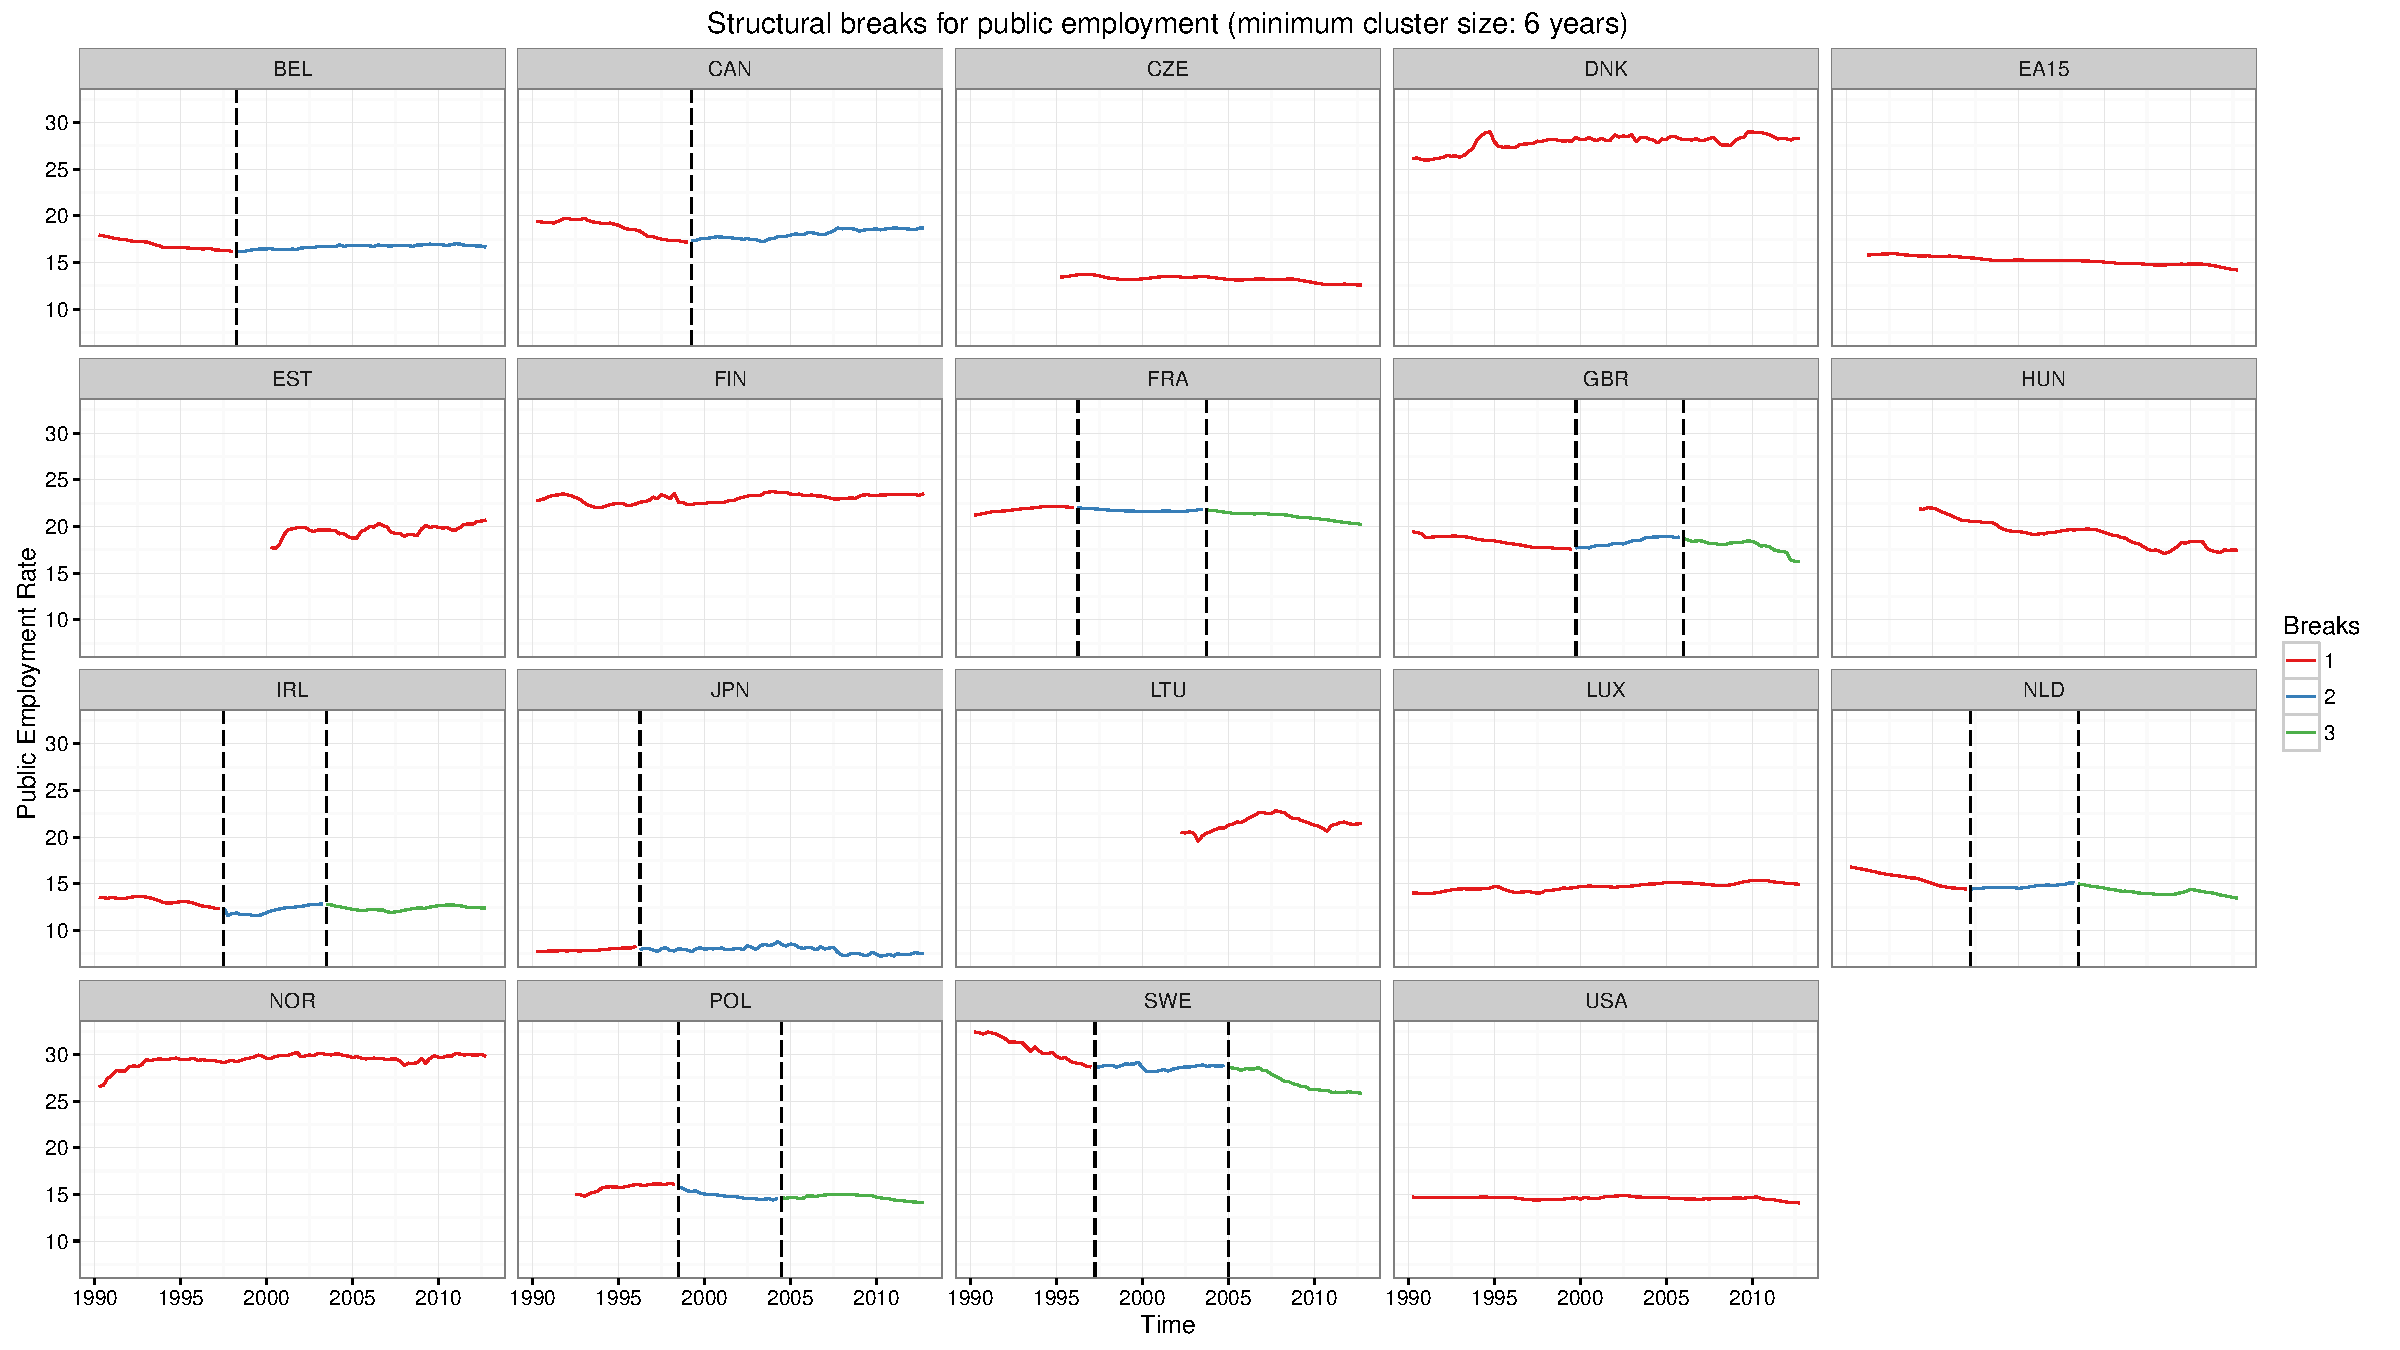
\includegraphics[width=1.5\textwidth]{tex_output/egr_structural_breaks}
  \caption{Structural breaks of the public employment rate using a
    non-parametric estimation of the breaks. Although there seems to have some
    breaks in individual countries, these do not justify a split in the
    analysis of the whole data set.}
  \label{fig:strct:breaks}
\end{figure}
\end{landscape}


\begin{figure}[!ht]
  \label{fig:diag:lm} \centering
  \includegraphics[width=\textwidth]{tex_output/model_diagnostic_quarterly}
  \caption{Diagnostic plots for the base line model. On the upper-left plot,
    one observes that the residuals are not uniformly distributed on the fitted
    values. The upper-right plot shows that the residuals are probably not
    distributed as a Gaussian variable as well. Hence some care should be taken
    with the assumption of the model and its output.}
\end{figure}

%%% Local Variables: ***
%%% mode:latex ***
%%% TeX-master: "semester_paper_sfs.tex" ***
%%% End: ***
%%% reftex-default-bibliography: ("biblio.bib")
 % empirical results % description of data set
\chapter{Conclusion}

In this semester paper, part of theory of data completion is reviewed. The main
work is devoted to build a framework to test several R packages for imputation
methods on the FLAS data set. With this data set, it appears that K-nearest
neighbor imputation works fairly well, although its implementation might throw
frustrating low level errors (segmentation faults). Except for
\texttt{softImpute}, all methods have the same order of error (distance between
the imputed and true value). In practice, they could unfortunately not be used
as black-box as most data matrix have collinear dimensions which constitutes an
issue for all the algorithms based on regression.

Finally, as departing words, one should not forget why these technique
exists. From \cite{schafer2002missing},

\begin{quote}
  With or without missing data, the goal of a statistical procedure should be
  to make valid and efficient inferences about a population of interest -- not to
  estimate, predict, or recover missing observations nor to obtain the same
  results that we would have seen with complete data.
\end{quote}


%%% Local Variables: ***
%%% mode:latex ***
%%% TeX-master: "semester_paper_sfs.tex"  ***
%%% End: ***
%%% reftex-default-bibliography: ("biblio.bib")


\linespread{1.0}\selectfont

%%%%%%%%%%%%%%%%%%%%%%%%%%%%%%%%%%%%%%%%%%%%%%%%%
%%% bibliography                              %%%
%%%%%%%%%%%%%%%%%%%%%%%%%%%%%%%%%%%%%%%%%%%%%%%%%
\addtocontents{toc}{\vspace{.5\baselineskip}}
\cleardoublepage
\phantomsection
\addcontentsline{toc}{chapter}{\protect\numberline{}{Bibliography}}
\bibliography{biblio}
%% all books from our library (sfs) are already in a bibtex file
%% (assbib). you can use assbib combined with your personal bibtex file:
%% \bibliography{myreferences,assbib}. of course, this will only work on
%% the computers at sfs, unless you copy the assbib file
%%  --> /u/sfs/bib/assbib.bib

%%%%%%%%%%%%%%%%%%%%%%%%%%%%%%%%%%%%%%%%%%%%%%%%%
%%% appendices (if needed)                    %%%
%%%%%%%%%%%%%%%%%%%%%%%%%%%%%%%%%%%%%%%%%%%%%%%%%
\addtocontents{toc}{\vspace{.5\baselineskip}}
\appendix
\chapter{Data visualizations}
\label{ch:data-viz}
The purpose of the following graphics is to offer some visual checks in order
to detect any anomalies in the data set.

\begin{landscape}
  \insertplot{simple_model_quarterly_gdpv_annpct.tex}{GDP growth, volume}
  \insertplot{simple_model_quarterly_unr.tex}{Unemployment rate}
  \insertplot{simple_model_quarterly_government_revenue.tex}{Government revenue in
    percent of GDP}
  \insertplot{simple_model_quarterly_gdp_per_capita_interpolated.tex}{GDP per
    Capita in USD millions}
  \insertplot{simple_model_quarterly_nlg_to_gdp.tex}{Net lending in
    percent of GDP}
\end{landscape}


\chapter{Regression tables}
\label{ch:reg-tbls}
This part provides the regression tables of the many regressions used to test
the different variables and to check the robustness of the base model, which
includes the unemployment rate, government revenues and net lending as main
variables.

\begin{landscape}


% Table created by stargazer v.5.2 by Marek Hlavac, Harvard University. E-mail: hlavac at fas.harvard.edu
% Date and time: Die, Mär 15, 2016 - 18:57:57
\begin{table}[!htbp] \centering 
  \caption{Effect of GDP} 
  \label{} 
\begin{tabular}{@{\extracolsep{5pt}}lcc} 
\\[-1.8ex]\hline 
\hline \\[-1.8ex] 
 & \multicolumn{2}{c}{\textit{Dependent variable:}} \\ 
\cline{2-3} 
\\[-1.8ex] & \multicolumn{2}{c}{Public employment rate} \\ 
\\[-1.8ex] & (1) & (2)\\ 
\hline \\[-1.8ex] 
 Government Revenue & 0.008$^{***}$ & 0.008$^{***}$ \\ 
  & (0.003) & (0.003) \\ 
  & & \\ 
 Net Lending in percent of GDP & $-$0.006$^{***}$ & $-$0.005$^{***}$ \\ 
  & (0.001) & (0.001) \\ 
  & & \\ 
 Unemployment rate & $-$0.009$^{***}$ & $-$0.009$^{***}$ \\ 
  & (0.002) & (0.002) \\ 
  & & \\ 
 GDP growth, YoY in percent & 0.004$^{**}$ &  \\ 
  & (0.002) &  \\ 
  & & \\ 
 Constant & 0.517$^{***}$ & 0.584$^{***}$ \\ 
  & (0.133) & (0.131) \\ 
  & & \\ 
\hline \\[-1.8ex] 
Auto-correlation effect & Yes & Yes \\ 
Time effect & Yes & Yes \\ 
Country effect & Yes & Yes \\ 
\hline \\[-1.8ex] 
Observations & 1,570 & 1,570 \\ 
R$^{2}$ & 0.999 & 0.999 \\ 
Adjusted R$^{2}$ & 0.999 & 0.999 \\ 
Residual Std. Error & 0.146 (df = 1456) & 0.146 (df = 1457) \\ 
F Statistic & 22,388.310$^{***}$ (df = 113; 1456) & 22,512.150$^{***}$ (df = 112; 1457) \\ 
\hline 
\hline \\[-1.8ex] 
\textit{Note:}  & \multicolumn{2}{r}{$^{*}$p$<$0.1; $^{**}$p$<$0.05; $^{***}$p$<$0.01} \\ 
\end{tabular} 
\end{table} 


% Table created by stargazer v.5.2 by Marek Hlavac, Harvard University. E-mail: hlavac at fas.harvard.edu
% Date and time: Die, Mär 15, 2016 - 18:18:25
\begin{table}[!htbp] \centering 
  \caption{Effect of GDP per Capita} 
  \label{} 
\begin{tabular}{@{\extracolsep{5pt}}lcc} 
\\[-1.8ex]\hline 
\hline \\[-1.8ex] 
 & \multicolumn{2}{c}{\textit{Dependent variable:}} \\ 
\cline{2-3} 
\\[-1.8ex] & \multicolumn{2}{c}{Public employment rate} \\ 
\\[-1.8ex] & (1) & (2)\\ 
\hline \\[-1.8ex] 
 Government Revenue & 0.006$^{**}$ & 0.006$^{**}$ \\ 
  & (0.003) & (0.003) \\ 
  & & \\ 
 Net Lending in percent of GDP & $-$0.004$^{***}$ & $-$0.004$^{***}$ \\ 
  & (0.001) & (0.001) \\ 
  & & \\ 
 Unemployment rate & $-$0.009$^{***}$ & $-$0.007$^{***}$ \\ 
  & (0.002) & (0.002) \\ 
  & & \\ 
 Log of GDP per capita, in USD Millions & $-$0.069 &  \\ 
  & (0.070) &  \\ 
  & & \\ 
 Constant & 1.330$^{*}$ & 0.586$^{***}$ \\ 
  & (0.765) & (0.131) \\ 
  & & \\ 
\hline \\[-1.8ex] 
Auto-correlation effect & Yes & Yes \\ 
Time effect & Yes & Yes \\ 
Country effect & Yes & Yes \\ 
\hline \\[-1.8ex] 
Observations & 1,449 & 1,449 \\ 
R$^{2}$ & 0.999 & 0.999 \\ 
Adjusted R$^{2}$ & 0.999 & 0.999 \\ 
Residual Std. Error & 0.145 (df = 1337) & 0.145 (df = 1338) \\ 
F Statistic & 22,321.440$^{***}$ (df = 111; 1337) & 22,524.810$^{***}$ (df = 110; 1338) \\ 
\hline 
\hline \\[-1.8ex] 
\textit{Note:}  & \multicolumn{2}{r}{$^{*}$p$<$0.1; $^{**}$p$<$0.05; $^{***}$p$<$0.01} \\ 
\end{tabular} 
\end{table} 


% Table created by stargazer v.5.2 by Marek Hlavac, Harvard University. E-mail: hlavac at fas.harvard.edu
% Date and time: Die, Mär 15, 2016 - 18:57:53
\begin{table}[!htbp] \centering 
  \caption{Effect of Years until next Election} 
  \label{} 
\begin{tabular}{@{\extracolsep{5pt}}lcc} 
\\[-1.8ex]\hline 
\hline \\[-1.8ex] 
 & \multicolumn{2}{c}{\textit{Dependent variable:}} \\ 
\cline{2-3} 
\\[-1.8ex] & \multicolumn{2}{c}{Public employment rate} \\ 
\\[-1.8ex] & (1) & (2)\\ 
\hline \\[-1.8ex] 
 Unemployment rate & $-$0.009$^{***}$ & $-$0.009$^{***}$ \\ 
  & (0.002) & (0.002) \\ 
  & & \\ 
 Government Revenue & 0.008$^{***}$ & 0.008$^{***}$ \\ 
  & (0.003) & (0.003) \\ 
  & & \\ 
 Net Lending in percent of GDP & $-$0.005$^{***}$ & $-$0.005$^{***}$ \\ 
  & (0.002) & (0.002) \\ 
  & & \\ 
 Years until next election & $-$0.004 &  \\ 
  & (0.003) &  \\ 
  & & \\ 
 Constant & 0.595$^{***}$ & 0.583$^{***}$ \\ 
  & (0.134) & (0.134) \\ 
  & & \\ 
\hline \\[-1.8ex] 
Auto-correlation effect & Yes & Yes \\ 
Time effect & Yes & Yes \\ 
Country effect & Yes & Yes \\ 
\hline \\[-1.8ex] 
Observations & 1,492 & 1,492 \\ 
R$^{2}$ & 0.999 & 0.999 \\ 
Adjusted R$^{2}$ & 0.999 & 0.999 \\ 
Residual Std. Error & 0.149 (df = 1379) & 0.149 (df = 1380) \\ 
F Statistic & 21,095.540$^{***}$ (df = 112; 1379) & 21,281.620$^{***}$ (df = 111; 1380) \\ 
\hline 
\hline \\[-1.8ex] 
\textit{Note:}  & \multicolumn{2}{r}{$^{*}$p$<$0.1; $^{**}$p$<$0.05; $^{***}$p$<$0.01} \\ 
\end{tabular} 
\end{table} 


% Table created by stargazer v.5.2 by Marek Hlavac, Harvard University. E-mail: hlavac at fas.harvard.edu
% Date and time: Mit, Jan 13, 2016 - 22:26:58
\begin{table}[!htbp] \centering 
  \caption{Effect of IMF GFS Score} 
  \label{} 
\begin{tabular}{@{\extracolsep{5pt}}lcc} 
\\[-1.8ex]\hline 
\hline \\[-1.8ex] 
 & \multicolumn{2}{c}{\textit{Dependent variable:}} \\ 
\cline{2-3} 
\\[-1.8ex] & \multicolumn{2}{c}{Public employment rate} \\ 
\\[-1.8ex] & (1) & (2)\\ 
\hline \\[-1.8ex] 
 GDP growth & $-$0.00002 & $-$0.00001 \\ 
  & (0.00003) & (0.00001) \\ 
  & & \\ 
 Unemployment rate & 0.002$^{***}$ & 0.002$^{***}$ \\ 
  & (0.0001) & (0.0001) \\ 
  & & \\ 
 Lagged Unemployment rate & $-$0.002$^{***}$ & $-$0.002$^{***}$ \\ 
  & (0.0001) & (0.0001) \\ 
  & & \\ 
 Government expenditure in \% of GDP (interpolated) & 0.00000 & 0.00000 \\ 
  & (0.00001) & (0.00001) \\ 
  & & \\ 
 Log of working population (interpolated) & $-$0.0001$^{***}$ & $-$0.0001$^{***}$ \\ 
  & (0.00003) & (0.00003) \\ 
  & & \\ 
 GDP per capita, in USD Millions (interpolated) & $-$0.000$^{***}$ & $-$0.000$^{***}$ \\ 
  & (0.000) & (0.000) \\ 
  & & \\ 
 Fiscal Transparency & $-$0.00000 &  \\ 
  & (0.00000) &  \\ 
  & & \\ 
 Effect of fiscal transparency on GDP growth & 0.00000 &  \\ 
  & (0.00000) &  \\ 
  & & \\ 
 Constant & 0.018$^{*}$ & 0.018$^{*}$ \\ 
  & (0.010) & (0.010) \\ 
  & & \\ 
\hline \\[-1.8ex] 
Year fixed-effect & Yes & Yes \\ 
Country fixed-effect & No & No \\ 
Auto-correlation effect & Yes & Yes \\ 
Quarter effect & Yes & Yes \\ 
\hline \\[-1.8ex] 
Observations & 2,496 & 2,496 \\ 
R$^{2}$ & 0.205 & 0.205 \\ 
Adjusted R$^{2}$ & 0.200 & 0.201 \\ 
Residual Std. Error & 0.002 (df = 2482) & 0.002 (df = 2484) \\ 
F Statistic & 49.091$^{***}$ (df = 13; 2482) & 58.062$^{***}$ (df = 11; 2484) \\ 
\hline 
\hline \\[-1.8ex] 
\textit{Note:}  & \multicolumn{2}{r}{$^{*}$p$<$0.1; $^{**}$p$<$0.05; $^{***}$p$<$0.01} \\ 
\end{tabular} 
\end{table} 

% Table created by stargazer v.5.2 by Marek Hlavac, Harvard University. E-mail: hlavac at fas.harvard.edu
% Date and time: Die, Mär 15, 2016 - 18:40:14
\begin{table}[!htbp] \centering
  \caption{Effect of Government Political Orientation}
  \label{}
\begin{tabular}{@{\extracolsep{5pt}}lcc}
\\[-1.8ex]\hline
\hline \\[-1.8ex]
 & \multicolumn{2}{c}{\textit{Dependent variable:}} \\
\cline{2-3}
\\[-1.8ex] & \multicolumn{2}{c}{Public employment rate} \\
\\[-1.8ex] & (1) & (2)\\
\hline \\[-1.8ex]
 Unemployment rate & $-$0.009$^{***}$ & $-$0.009$^{***}$ \\
  & (0.002) & (0.002) \\
  & & \\
 Government Revenue & 0.007$^{***}$ & 0.008$^{***}$ \\
  & (0.003) & (0.003) \\
  & & \\
 Net Lending in percent of GDP & $-$0.005$^{***}$ & $-$0.005$^{***}$ \\
  & (0.002) & (0.002) \\
  & & \\
 Government with a left-wing partisanship & 0.014 &  \\
  & (0.011) &  \\
  & & \\
 Constant & 0.601$^{***}$ & 0.583$^{***}$ \\
  & (0.134) & (0.134) \\
  & & \\
\hline \\[-1.8ex]
Auto-correlation effect & Yes & Yes \\
Time effect & Yes & Yes \\
Country effect & Yes & Yes \\
\hline \\[-1.8ex]
Observations & 1,492 & 1,492 \\
R$^{2}$ & 0.999 & 0.999 \\
Adjusted R$^{2}$ & 0.999 & 0.999 \\
Residual Std. Error & 0.149 (df = 1379) & 0.149 (df = 1380) \\
F Statistic & 21,103.400$^{***}$ (df = 112; 1379) & 21,281.620$^{***}$ (df = 111; 1380) \\
\hline
\hline \\[-1.8ex]
\textit{Note:}  & \multicolumn{2}{r}{$^{*}$p$<$0.1; $^{**}$p$<$0.05; $^{***}$p$<$0.01} \\
\end{tabular}
\end{table}


% Table created by stargazer v.5.2 by Marek Hlavac, Harvard University. E-mail: hlavac at fas.harvard.edu
% Date and time: Die, Mär 15, 2016 - 18:57:54
\begin{table}[!htbp] \centering 
  \caption{Effect of Gini coefficient, data up to 2010 (included)} 
  \label{} 
\begin{tabular}{@{\extracolsep{5pt}}lcc} 
\\[-1.8ex]\hline 
\hline \\[-1.8ex] 
 & \multicolumn{2}{c}{\textit{Dependent variable:}} \\ 
\cline{2-3} 
\\[-1.8ex] & \multicolumn{2}{c}{Public employment rate} \\ 
\\[-1.8ex] & (1) & (2)\\ 
\hline \\[-1.8ex] 
 Unemployment rate & $-$0.012$^{***}$ & $-$0.012$^{***}$ \\ 
  & (0.003) & (0.002) \\ 
  & & \\ 
 Government Revenue & 0.013$^{***}$ & 0.012$^{***}$ \\ 
  & (0.003) & (0.003) \\ 
  & & \\ 
 Net Lending in percent of GDP & $-$0.008$^{***}$ & $-$0.007$^{***}$ \\ 
  & (0.002) & (0.002) \\ 
  & & \\ 
 Gini Coefficient, Market Income & $-$0.005 &  \\ 
  & (0.003) &  \\ 
  & & \\ 
 Gini Coefficient, Net Income & 0.010$^{**}$ &  \\ 
  & (0.005) &  \\ 
  & & \\ 
 Constant & 0.539$^{***}$ & 0.617$^{***}$ \\ 
  & (0.178) & (0.152) \\ 
  & & \\ 
\hline \\[-1.8ex] 
Auto-correlation effect & Yes & Yes \\ 
Time effect & Yes & Yes \\ 
Country effect & Yes & Yes \\ 
\hline \\[-1.8ex] 
Observations & 1,276 & 1,276 \\ 
R$^{2}$ & 0.999 & 0.999 \\ 
Adjusted R$^{2}$ & 0.999 & 0.999 \\ 
Residual Std. Error & 0.151 (df = 1174) & 0.151 (df = 1176) \\ 
F Statistic & 19,893.780$^{***}$ (df = 101; 1174) & 20,255.620$^{***}$ (df = 99; 1176) \\ 
\hline 
\hline \\[-1.8ex] 
\textit{Note:}  & \multicolumn{2}{r}{$^{*}$p$<$0.1; $^{**}$p$<$0.05; $^{***}$p$<$0.01} \\ 
\end{tabular} 
\end{table} 


\end{landscape}


\chapter{R Implementation Details}
\label{app:complement}

The complete \textsf{R} code to generate the results is stored on
\url{https://github.com/davidpham87/public_employment_analysis} where the
procedures are more documented. The first script provides some functions useful
for the analysis, the second displays how the data were manipulated to create
the data matrix, whereas the third is used to produce the results.

\paragraph{Initialization script} \ \vspace{10pt}

\lstinputlisting[language=R, style=Rstyle]{../../PublicEmploymentAnalysis/R/init.R}

\paragraph{Data manipulation script} \ \vspace{10pt}

\lstinputlisting[language=R, style=Rstyle]{../../PublicEmploymentAnalysis/R/data_preparation.R}

\paragraph{Analysis script} \ \vspace{10pt}

\lstinputlisting[language=R, style=Rstyle]{../../PublicEmploymentAnalysis/R/eda_quarterly_new_data.R}


%%% Local Variables:
%%% mode: latex
%%% TeX-master: "semester_paper_sfs"
%%% End:


% %% epilogue (optional)
% \addtocontents{toc}{\vspace{.5\baselineskip}}
% \cleardoublepage
% \phantomsection
% \addcontentsline{toc}{chapter}{\protect\numberline{}{Epilogue}}
% \markboth{Epilogue}{Epilogue}

%%%%%%%%%%%%%%%%%%%%%%%%%%%%%%%%%%%%%%%%%%%%%%%%%%
%%% Declaration of originality (Do not remove!)%%%
%%%%%%%%%%%%%%%%%%%%%%%%%%%%%%%%%%%%%%%%%%%%%%%%%%
%% Instructions:
%% -------------
%% fill in the empty document confirmation-originality.pdf electronically
%% print it out and sign it
%% scan it in again and save the scan in this directory with name
%% confirmation-originality-scan.pdf
%%
%% General info on plagiarism:
%% https://www.ethz.ch/students/en/studies/performance-assessments/plagiarism.html
\cleardoublepage
\includepdf[pages={-}, frame=true,scale=1]{confirmation-originality-scan.pdf}
\end{document}
